% This is samplepaper.tex, a sample chapter demonstrating the
% LLNCS macro package for Springer Computer Science proceedings;
% Version 2.20 of 2017/10/04
%
\documentclass[runningheads]{llncs}

\pagestyle{plain}
% needed by SAC to show page numbers
%
% need to remove before submission
\usepackage[colorlinks]{hyperref}

\usepackage{graphicx}
\usepackage[utf8]{inputenc}
% *** MATH PACKAGES ***
%
\usepackage{amsmath}
\usepackage{listings}% use mathematical symbols in Verbatim environment
\lstset{
  basicstyle=\ttfamily,
  mathescape
}
\usepackage{amsfonts,amssymb}
%\usepackage[linesnumbered,ruled,vlined]{algorithm2e}
\usepackage[linesnumbered,boxed,vlined]{algorithm2e}
% *** ALIGNMENT PACKAGES ***
%
\usepackage{array}
% *** PDF, URL AND HYPERLINK PACKAGES ***
%
\usepackage{url}



%personal defined packages
\usepackage{multirow,array}
% *** TABLE FOOTNOTE PACKAGES ***
\usepackage[bottom]{footmisc}
\usepackage{footnote}
\makeatletter
\def\@xfootnote[#1]{%
  \protected@xdef\@thefnmark{#1}%
  \@footnotemark\@footnotetext}
\makeatother
\usepackage{threeparttable}

\usepackage{caption}
\usepackage{subcaption}
\captionsetup{compatibility=false}

\usepackage{placeins}

 %table dash line
\usepackage{arydshln}

\usepackage{morefloats}

\begin{document}
%
\title{FPGA-Based Key Generator for Post-Quantum Key Encapsulation Based on Quasi-Cyclic Codes}
%
%\titlerunning{Abbreviated paper title}
% If the paper title is too long for the running head, you can set
% an abbreviated paper title here
%
% \author{Jingwei Hu\inst{1} \and Wen Wang\inst{2} \and Ray Cheung\inst{3} \and San Ling\inst{1} \and Huaxiong Wang\inst{1}}



% \authorrunning{Jingwei Hu \textit{et. al.}}
% % First names are abbreviated in the running head.
% % If there are more than two authors, 'et al.' is used.
% %


% \institute{School of Physical and Mathematical Sciences, Nanyang Technological University, Singapore, \email{\{davidhu, lingsan, HXWang\}@ntu.edu.sg}
% \and Department of Electrical Engineering, Yale University, USA,\\ \email{wen.wang.ww349@yale.edu}
% \and Department of Electronic Engineering, City University of Hong Kong, Hong Kong, \email{r.cheung@cityu.edu.hk} }
% %
\maketitle              % typeset the header of the contribution
%


\begin{abstract}
In this paper, we present a constant-time FPGA-based key generator for a
quantum-safe key encapsulation mechanism based on MDPC codes
called BIKE,
which is among round-2 candidates in the NIST PQC standardization process.
Existing hardware implementations of MDPC code-based systems
focus on the encryption/decryption (key encapsulation/decapsulation)
operations while few of them take into account
the key generation operation which is particularly crucial for
KEM-based applications.
The hardware architecture for the key generator
proposed in this work
aims at maximizing the metric of timing efficiency
while maintaining a low resource consumption.
% under a given resource restriction. New
Parallelized polynomial multiplication and squaring
algorithms are proposed
and implemented to achieve this goal.
Our experimental results show that our key generator design
% with 128-bit post-quantum security
requires $9.5\times 10^5$ cycles (0.597 ms),
$2.1\times 10^6$ cycles (14.334 ms) and $9.8\times 10^5$ cycles (0.492 ms)
respectively
to generate a key pair for BIKE-1/2/3.
The proposed key generator is very area-efficient,
it uses only $544/1272/423$ slices for BIKE-1/2/3 on
a small-sized low-end Xilinx Spartan-7 FPGA.

\keywords{Post-Quantum Cryptography, Key Encapsulation Mechanism, Key Generator, QC-MDPC Code, FPGA Implementation}
\end{abstract}
%
%
%
\section{Introduction}
Key encapsulation mechanisms (KEMs) are commonly used encryption techniques
to secure the transmission of symmetric cryptographic keys
by use of public-key cryptographic algorithms.
Therefore, efficient and secure KEM designs have always been an important topic
in the cryptographic community.
In the past few years, NIST has started the PQC standardization process
soliciting the designs of efficient and secure post-quantum KEMs~\cite{chen2016report}
since the construction of a commercial quantum computer emerges as an urgent
threat to the commonly used cryptographic primitives nowadays.
These primitives rely on the hardness of the integer factorization problem or
discrete logarithm problems, e.g., the Diffie-Hellman key exchange,
the Rivest-Shamir-Adleman (RSA) and Elliptic Curve Cryptography (ECC).
However, in 1994 Shor's algorithm \cite{shor1997polynomial} was proposed
which can be deployed
on a quantum computer and solve both the integer factorization problem
and the discrete logarithm problem in polynomial time, and therefore will
render the security of the modern cryptographic primitives.

Code-based cryptosystems, which build their security on the hardness of
decoding general linear codes, are among the most promising quantum-secure
candidates for which no known polynomial time attacks exist by use of a quantum computer.
McEliece proposed the first code-based cryptosystem in 1978 \cite{mceliece1978public},
which uses binary Goppa codes \cite{goppa1970new} in the underlying coding system.
However, Goppa code-based schemes yield large public keys which limit
the deployment of these systems in resource-constrained scenarios.
Niederreiter proposed in 1986 a variant of the McEliece cryptosystem~\cite{niederreiter1986knapsack}
which introduced a trick to reduce the size of the public key,
namely the Niederreiter cryptosystem.
% which exploits the same trapdoor function.
% The Niederreiter cryptosystem uses the syndromes and parity-check matrices to construct the ciphertext and the key.
It has been proven that the Niederreiter cryptosystem and the McEliece cryptosystem
achieve the same security level~\cite{li1994equivalence} when the same family of codes is used.

Active research has been focused on replacing Goppa codes
with other families of structured codes for reducing the key size.
Nevertheless, many of these attempts lead to the compromise of the the system security.
For example, many McEliece variants based on low-density parity-check (LDPC) codes~\cite{monico2000using},
quasi-cyclic low-density parity-check (QC-LDPC) codes \cite{otmani2010cryptanalysis},
quasi-dyadic (QD) codes \cite{misoczki2009compact},
convolutional codes \cite{londahl2012new}, generalized Reed-Solomon (GRS) codes \cite{baldi2016enhanced}, and rank-metric codes \cite{loidreau2017new,gaborit2018polynomial}
have been successfully broken.
However, a few variants exploiting the quasi-cyclic form of the codes~\cite{baldi2013optimization,baldi2008new,misoczki2013mdpc} have been shown to counteract
all the existing cryptanalysis attacks while maintaining small-sized keys.
A variety of KEMs built on the Niederreiter cryptosystem and LDPC/MDPC codes
such as LEDAkem \cite{baldi2018ledakem}, CAKE \cite{barreto2017cake} and BIKE \cite{aragon2017bike}
are proposed and analyzed in the literature.
Among these proposals, BIKE is currently
among the round-2 candidates for the NIST PQC standardization process.
Recently, a new statistical attack, called reaction attack \cite{fabvsivc2017reaction,guo2016key}
has been devised to recover the key by exploiting the information leaked from decoding failures in QC-LDPC and QC-MDPC code-based systems.
This attack is further enhanced in \cite{nilsson2019error} where the error pattern chaining method
is introduced to generate multiple undecodable error patterns from an initial error pattern,
thus improving the performance of such reaction attack in the CPA case.
However, the reaction attack only works for CPA systems and long-term keys, therefore,
the deployment of a CCA2-secure conversion or ephemeral keys in BIKE
can resist the attack.


\paragraph{Contributions.} Most of the existing work on hardware implementations of MDPC code-based
cryptosystems focus on the encryption and decrption operations.
% However, it should be considered to have a closer look at the
% key generation as well.
However, KEMs are gradually getting more commonly used in ephemeral
key encapsulation scenarios in which cases the key
generation is used as often as the encapsulation and decapsulation operations
and therefore should also be accelerated by dedicated hardware modules.
% we do have a strong motivation to accelerate the key generation since KEMs use ephemeral keys which require updating keys frequently.
Therefore, in this work we present the first constant-time, efficient and compact
FPGA-based key generator for a promising MDPC code-based post-quantum KEM \mbox{---} BIKE.
Our contributions include:
\begin{itemize}
  \item The proposal of new polynomial arithmetic algorithms (squaring, generic polynomial multiplication and sparse polynomial multiplication) over ring $\mathbb{F}_2[x]/\langle x^r+1\rangle$.
  \item Constant-time and efficient hardware architectures for the polynomial arithmetics
  in $\mathbb{F}_2[x]/\langle x^r+1\rangle$ including polynomial inversion, polynomimal squaring, polynomial multiplications and
  polynomial generation.
  % \item The timing scores ($9.55 \times 10^4$, $2.15 \times 10^6$, and $9.85 \times 10^4$ clock cycles for BIKE-1, BIKE-2, and BIKE-3, respectively) of our design outperform other embedded hardware and even powerful CPU with the dedicate carry-less multiplication instruction in terms of cycle count.
  \item Novel and lightweight hardware architectures for the key generator of three BIKE variants of security ranging
  between 128-bit and 256-bit.
\end{itemize}

% \paragraph{Outline.}
% The paper is organized as follows.
% In Section~\ref{sec::prelim}, we describe the basic notations
% and introduce the related aspects of the BIKE cryptosystem.
% Later in Section~\ref{sec::modules}, we present the design methodologies
% for implementing the arithmetics in BIKE efficiently
% on reconfigurable devices.
% In particular, new algorithms for
% polynomial multiplications and squaring are proposed and
% the design details are presented.
% %to achieve time efficiency and area efficiency.
% In Section~\ref{sec::keygen}, a generic lightweight architecture for the key generator of BIKE
% is presented.
% Experimental results on Xilinx FPGAs are shown to demonstrate the
% efficiency of the proposed algorithms and hardware architectures
% in Section~\ref{sec::evaluation}.
% Finally, conclusions are drawn in Section~\ref{sec::conclusion}.

% \section{Preliminaries for BIKE/LEDAkem Key Generation}
\section{Preliminaries}
\label{sec::prelim}

In the following, we describe the basic notations and definitions
in QC-MDPC codes which closely follow the descriptions in~\cite{aragon2017bike}. Quasi-cyclic (QC) codes can be  defined  over either matrices or polynomial rings.
We use both the matrix view and the polynomial view to
describe the relevant aspects of the BIKE scheme.
% scheme better.


\newcommand{\tabincell}[2]{\begin{tabular}{@{}#1@{}}#2\end{tabular}}
%\begin{table*}[!t]\centering
%\caption{Parameters for LEDAkem according to NIST defined security category, referenced from \cite{baldi2018ledakem}}
%\label{table:systempar}
%\begin{minipage}{\textwidth}\centering
%\begin{tabular}{cc|cccccc}
%\hline
%\tabincell{c}{\textbf{Category}} &  $\mathbf{n_0}$ & $\mathbf{r}$ & $\mathbf{w}$ & \textbf{[$m_0,\cdots,m_{n_0-1}$]} & \textbf{t} & \textbf{SL} & \textbf{DFR}\\
%\hline
%\multirow{ 3}{*}{1} & 2 & 15,013 & 9 & [5,4] & 143 & \multirow{ 3}{*}{128} & $\leq 10^{-9}$\\
%                    & 3 & 9,643 & 13 & [3,2,2]&90 &                       & $\approx 10^{-9}$\\
%                    & 4 & 8,467 & 11 & [3,2,2,2]&72 &                     & $\approx 10^{-9}$\\
%\hline
%\multirow{ 3}{*}{2-3} & 2 & 24,533 & 13 & [5,4] & 208 & \multirow{ 3}{*}{192} & $\leq 10^{-8}$\\
%                      & 3 & 17,827 & 15 & [4,3,2]&129 &                       & $\leq 10^{-8}$\\
%                      & 4 & 14,717 & 15 & [3,2,2,2]&104 &                     & $\leq 10^{-8}$\\
%\hline
%\multirow{ 3}{*}{4-5} & 2 & 37,619 & 11 & [7,6] & 272 & \multirow{ 3}{*}{256} & $\leq 10^{-8}$\\
%                      & 3 & 28,477 & 13 & [5,4,4]&172 &                       & $\leq 10^{-8}$\\
%                      & 4 & 22,853 & 13 & [4,3,3,3]&135 &                     & $\leq 10^{-8}$\\
%\hline
%\end{tabular}
%\end{minipage}
%\end{table*}

\subsection{General Definitions}

Table~\ref{tab::definition} shows the notations
used in the following discussions.

\begin{table}[!tbh]
  \centering
  \begin{tabular}{ll}
     \hline
     % after \\: \hline or \cline{col1-col2} \cline{col3-col4} ...
     Polynomial View: &\\
     $\mathbb{F}_2$ & Finite field of 2 elements \\
     $\mathcal{R}$ & The cyclic polynomial ring $\mathbb{F}_2[x]/\langle x^r+1\rangle$\\
     $|x|$ & The Hamming weight of a binary polynomial $x$ \\
     $u \overset{\underset{\$}{}}{\gets} U$ & Variable $u$ is sampled uniformly at random from set $U$ \\
     \hline
     Matrix View: &\\
     $\mathcal{V}$ & The vector space of dimension $n$ over $\mathbb{F}_2$\\
     $\mathbf{m}$ & The vector over $\mathbb{F}_2$\\
     $\mathbf{G}$ & The matrix over $\mathbb{F}_2$\\
     \hline
   \end{tabular}
  \caption{Notations}\label{table:notation}
  \label{tab::definition}
\vspace{-4mm}
\end{table}
%
The basic structure in QC codes is the circulant matrix,
which is defined as follows:
\begin{definition}{(Circulant Matrix)}
Let $\mathbf{x}=(x_0,\ldots,x_{n-1})\in \mathbb{F}_2^n$. The circulant matrix induced by $\mathbf{x}$ is defined and denoted as follows:
\[
 \mathbf{rot(x)} = \left[ \begin{array}{cccc}
        x_0 & x_{n-1} & \cdots &x_{1}\\
        x_{1} & x_{0} & \cdots &x_{2}\\
        \vdots & \vdots & \ddots & \vdots \\
        x_{n-1} & x_{n-2} & \cdots & x_{0}
        \end{array}\right ]
\]
\end{definition}
%
Therefore, the product of any two polynomials $x$ and $y$ in $\mathcal{R}$ can be viewed as a vector-matrix (or matrix-vector) product using the operator $\mathbf{rot(\cdot)}$ as:
\[
   x\cdot y=\mathbf{x}\cdot \mathbf{rot(y)}^T=\mathbf{y}\cdot \mathbf{rot(x)}^T=y\cdot x
\]
%
MDPC codes are a special variant of linear codes and are defined as follows:
\begin{definition}{(Linear Code)}
A Binary Linear Code $\mathcal{C}$ of length $n$ and dimension $k$ (denoted as $[n,k]$) is a subspace of $\mathcal{V}$ of dimension $k$. Elements of $\mathcal{C}$ are referred to as codewords.
\end{definition}

\begin{definition}{(Generator and Parity-Check Matrix)}
$\mathbf{G}\in \mathbb{F}^{k\times n}$ is a Generator Matrix for the $[n,k]$ code $\mathcal{C}$ iff
\[
\mathcal{C}=\{\mathbf{mG}|\mathbf{m}\in \mathbb{F}_2^k\}
\]

$\mathbf{H}\in \mathbb{F}^{(n-k)\times n}$ is called a Parity-Check Matrix of $\mathcal{C}$ iff
\[
\mathcal{C}=\{\mathbf{c} \in \mathbb{F}_2^n |\mathbf{Hc}^T=0\}
\]
\end{definition}
%
A linear code can be quasi-cyclic according to the following definition:

\begin{definition}{(Quasi-Cyclic Codes)}
A binary quasi-cyclic (QC) code of index $n_0$ and order $r$ is a linear code which admits as generator matrix a block-circulant matrix of order $r$ and index $n_0$.
A ($n_0,k_0$)-QC code is a quasi-cyclic code of index $n_0$, length $n_0r$ and dimension $k_0r$
\end{definition}
%
For instance, the generator matrix of a $(3,1)$-QC code is formed by three circulant blocks $\mathbf{G_i}$:
$
\mathbf{G}=[\mathbf{G_0}|\mathbf{G_1}|\mathbf{G_2}]
$.

In the polynomial view, each block $\mathbf{G_i}$ can be represented (one-to-one mapping) as a polynomial $g_i$ over $\mathcal{R}$ and thus the generator matrix $\mathbf{G}$ can be viewed as the polynomial matrix $[g_0|g_1|g_2]$ over $\mathcal{R}$. In all aspects, any codeword $\mathbf{c}=\mathbf{m}\cdot\mathbf{G}$ over $\mathbb{F}^{n}$ can be represented in its polynomial form as $[mg_0|mg_1|mg_2]$ over $\mathcal{R}$. All the above notations are collected in
Table~\ref{table:notation}.


\subsection{BIKE}
%
BIKE was proposed by Aragon \textit{et. al} in 2017~\cite{aragon2017bike},
which is a novel code-based key encapsulation mechanism based on QC-sMDPC codes.
% called BIKE~\cite{aragon2017bike}, was submitted by Aragon \textit{et. al} in 2017.
The use of a QC-MDPC code $C(n_0,k_0)$ in BIKE brings a big key size reduction
compared to unstructured codes.
BIKE uses the double-circulant structure for the parity check matrix
where two smaller cyclic matrices are included.
Nine instances of BIKE (BIKE-1, BIKE-2, BIKE-3) are proposed
in their specification.
BIKE-1 is a variant which provides fast key generation
by using a variation of the McEliece cryptosystem.
A preliminary version of BIKE-1 first appeared in \cite{barreto2017cake}.
BIKE-2 follows Niederreiter's framework by use of
a systematic parity check matrix which can yield a very compact formulation.
The BIKE-3 variant follows the work of Ouroboros \cite{deneuville2017ouroboros}, featuring fast, inversion-less key generation operations.
The main difference in BIKE-3 is that the decapsulation invokes the decoding algorithm on a noisy syndrome. This also suggests that BIKE-3 is fundamentally distinct from BIKE-1 and BIKE-2 in terms of security aspects.
Parameters for these BIKE instances are shown in Table~\ref{table:systempar},
which covers the 5 security categories suggested by the NIST PQC standardization process.
QC construction of the codes brings a significant reduction
in memory storage required for public keys,
since only the first row/column of each circulant block
needs to be stored and the remaining part can be
reconstructed by cyclic rotations of the first row/column,
thus largely minimizing the public key size. % to be comparable with other post-quantum cryptographic candidates.
% BIKE currently is one of the second round candidate algorithms of the NIST post-quantum standardization project.

\begin{table*}[!t]\centering
\caption{Parameters for BIKE, referenced from \cite{aragon2017bike}}
\label{table:systempar}
\begin{minipage}{\textwidth}\centering
\begin{tabular}{cc|cccccc}
\hline
\tabincell{c}{\textbf{Category}} &  & $\mathbf{n}$ & $\mathbf{r}$ & $\mathbf{w}$ & \textbf{t} & \textbf{SL} & \textbf{DFR}\\
\hline
\multirow{ 2}{*}{1} & BIKE-[1,2] & 20,326 & 10,163 & 142 & 134 & \multirow{ 2}{*}{128} & \multirow{ 2}{*}{$\leq 10^{-7}$}\\
                    & BIKE-3 & 22,054 & 11,027 & 134 & 154 &                       & \\
\hline
\multirow{ 2}{*}{2-3} & BIKE-[1,2] & 39,706 & 19,853 & 206 &199 & \multirow{ 2}{*}{192} & \multirow{ 2}{*}{$\leq 10^{-7}$}\\
                      & BIKE-3 & 43,366 & 21,683 & 198 &226 &                       & \\
\hline
\multirow{ 2}{*}{4-5} & BIKE-[1,2] & 65,498 & 32,749 & 274 & 264 & \multirow{ 2}{*}{256} & \multirow{ 2}{*}{$\leq 10^{-7}$}\\
                      & BIKE-3 & 72,262 & 36,131 & 266 &300 &                       & \\
\hline
\end{tabular}
\end{minipage}
\vspace{-4mm}
\end{table*}

The key generation algorithms of BIKE-1/2/3 are described in the following text.
Algorithm~\ref{alg:bike1_keygen} describes the key generation algorithm of BIKE-1. The private keys comprise of two ``sparse'' polynomials $h_0$ and $h_1$ where $|h_0|$ and $|h_1|$ is restricted to $w/2$. The public keys $(f_0,f_1)$ are exposed for public use and therefore must be scrambled to hide the structure of $h_0$ and $h_1$. This is done by multiplying $h_0$ and $h_1$ by a random dense polynomial $g$ to get $gh_0$ and $gh_1$.


\begin{algorithm}[!tbh]
 \DontPrintSemicolon % Some LaTeX compilers require you to use \dontprintsemicolon instead
 \KwIn{$\lambda$, the target quantum security level.}
 \KwOut{the sparse private key $\mathbf{PK}=(h_0,h_1)$ and the dense public key $\mathbf{SK}=(f_0,f_1)$}
    Given $\lambda$, set the parameters $r,w$ as described above\;
    Generate $h_0,h_1 \gets \mathcal{R}$ both of (odd) weight $|h_0|=|h_1|=w/2$\;
    Generate $g \gets \mathcal{R}$ of odd weight (so $|g|\approx r/2$)\;
    Compute ($f_0,f_1$)$\gets$ ($gh_1,gh_0$)\;
    \Return {PK and SK\;}
 \caption{BIKE-1 key generation algorithm in polynomial view \cite{aragon2017bike}}\label{alg:bike1_keygen}
\end{algorithm}

\begin{algorithm}[!tbh]
 \DontPrintSemicolon % Some LaTeX compilers require you to use \dontprintsemicolon instead
 \KwIn{$\lambda$, the target quantum security level.}
 \KwOut{the sparse private key $\mathbf{PK}=(h_0,h_1)$ and the dense public key $\mathbf{SK}=h$}
    Given $\lambda$, set the parameters $r,w$ as described above\;
    Generate $h_0,h_1 \gets \mathcal{R}$ both of (odd) weight $|h_0|=|h_1|=w/2$\;
    Compute $h$ $\gets$ $h_1h_0^{-1}$\;
    \Return {PK and SK\;}
 \caption{BIKE-2 key generation algorithm in polynomial view  \cite{aragon2017bike}}\label{alg:bike2_keygen}
\end{algorithm}

\begin{algorithm}[!tbh]
 \DontPrintSemicolon % Some LaTeX compilers require you to use \dontprintsemicolon instead
 \KwIn{$\lambda$, the target quantum security level.}
 \KwOut{the sparse private key $\mathbf{PK}=(h_0,h_1)$ and the dense public key $\mathbf{SK}=(f_0,f_1)$}
    Given $\lambda$, set the parameters $r,w$ as described above\;
    Generate $h_0,h_1 \gets \mathcal{R}$ both of (odd) weight $|h_0|=|h_1|=w/2$\;
    Generate $g \gets \mathcal{R}$ of odd weight (so $|g|\approx r/2$)\;
    Compute ($f_0,f_1$)$\gets$ ($h_1+gh_0,g$)\;
    \Return {PK and SK\;}
 \caption{BIKE-3 key generation algorithm in polynomial view  \cite{aragon2017bike}}\label{alg:bike3_keygen}
\end{algorithm}


Algorithm~\ref{alg:bike2_keygen} describes the BIKE-2 key generation algorithm. Note that BIKE-2 does not generate any random polynomial to hide the secret keys $h_0$ and $h_1$. Instead, it computes $h=h_0^{-1}h_1$ as the public key.
 % by using polynomial inverse.
Therefore, the public key size is halved, however, the computational cost
increases due to the required polynomial inversion operation.

Algorithm~\ref{alg:bike3_keygen} describes the key generation algorithm of BIKE-3,
which is an improved version of BIKE-1.
% To further improve BIKE-1,
BIKE-3 uses only one multiplication and one addition to compute the first half of public key $f_0=h_1+gh_0$. The second half $f_1$ equals to the random dense polynomial $g$.
 % which requires no multiplication to compute.

\section{Polynomial Arithmetics}
\label{sec::modules}
In this section, we introduce the basic polynomial arithmetics
in $\mathbb{F}_2[x]/(x^r+1)$
for building the BIKE key generation architecture.
Algorithms and implementations for
polynomial squaring and multiplications,
polynomial inversion,
and generation of sparse/dense polynomials with prescribed Hamming weight
are presented in the following sub-sections.
% In particular, we thoroughly describe 1. the memory organization for polynomials used in BIKE 2. constant-time yet fast polynomial inverse, squaring and  multiplication algorithms used in BIKE 3. efficient generation of sparse/dense polynomials with prescribed Hamming weight.


\paragraph{Polynomial Representations.}
In this paper, two formats are used to represent polynomials in
the quotient ring $\mathbb{F}_2[x]/(x^r+1)$.
One is the dense format which stores all the coefficients
of a given polynomial $f=f_0+f_1x+\ldots +f_{r-1}x^{r-1}$. %in sequence.
This format is used when the polynomial is dense, e.g.,
the public keys $(f_0, f_1)$ are dense polynomials
and therefore are described in this format.
% For FPGA-based implementations, the coefficients $f_i$ of $f$ are typically stored in block RAMs, each address of which keeps multiple bits (word) of data. Let us define such data structure for a polynomial $f$ as $\overline{\mathbf{f}}$ where $\overline{\mathbf{f}[i]}$ denotes the word ($d$ bits in total) stored in the $i$-th address:
In our design, the coefficients of the polynomials are
stored in block RAMs, in which each address keeps multiple coefficients as a word.
Small endian notation is used here, \textit{i.e.}, $f_0$ is first stored, then $f_1$, and finally $f_{r-1}$.
% of data.
We define such data structure for a polynomial $f$ as $\overline{\mathbf{f}}$
where $\overline{\mathbf{f}[i]}$ denotes the word ($d$ bits in total) stored in the $i$-th address as: $(f_{id},f_{id+1},\ldots,f_{id+d-1})_2$.
By using this format, in total $\lceil r/d \rceil$ words
are needed to represent a polynomial over $\mathbb{F}_2[x]/(x^r+1)$.
For the last word  $\mathbf{\overline{f}}[\lceil r/d \rceil-1]$,
we append a few zeros to fill it as a complete word:
$(f_{(\lceil r/d\rceil-1)d},\ldots, f_{r},\ldots,0)_2$.
Figure~\ref{fig:poly_dense} illustrates the data structure of $\overline{\mathbf{f}}$.

The other format is the sparse format which is used
when the polynomial is sparse, e.g.,
the secret keys $(h_0, h_1)$.
This format only saves the bit positions of non-zero coefficients in a polynomial $f$.
% For example, the secret keys $(h_0, h_1)$ are sparse polynomials and can be described well by the sparse format.
We define this sparse form for a polynomial $f$ as $\mathbf{\hat{f}}$ where
$\hat{\mathbf{f}[i]}$ denotes the non-zero bit position (belongs to the set $\{i|f_i=1\}$, each item of this set is $log_2(r)$ bits) stored in the $i$-th address.
This format is memory-efficient especially when
the weight of $f$ is small:
It takes $|f|$ words and each word is of $log_2(r)$ bits to
represent a given polynomial $f$. % if the polynomial weight is small.
Figure~\ref{fig:poly_sparse} illustrates the data structure of $\mathbf{\hat{f}}$.

\begin{figure*}[!tb]
\centering
\begin{subfigure}[t]{0.43\textwidth}\centering
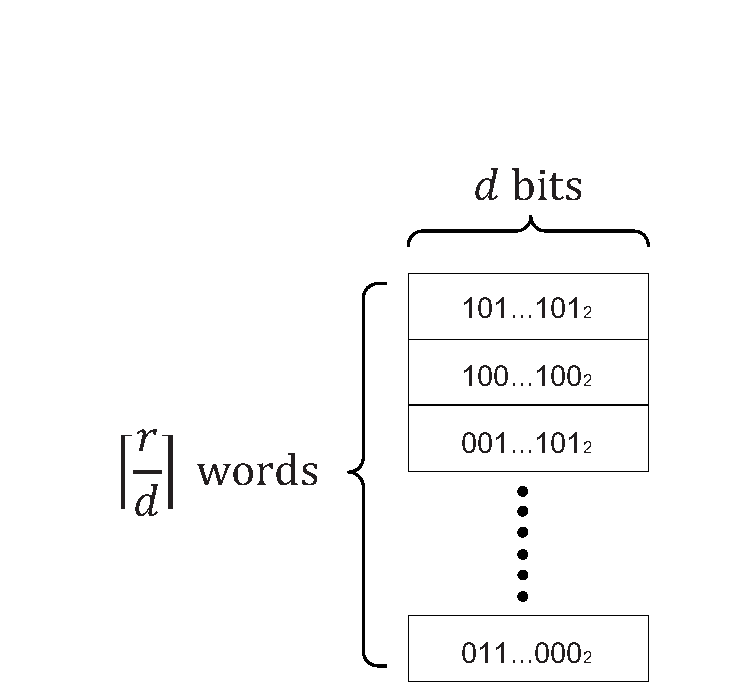
\includegraphics[width=\textwidth]{./fig/PolyDenseFormat.eps}
\caption{Polynomial represented in dense Format}
\label{fig:poly_dense}
\end{subfigure}
\hspace{1em}
\begin{subfigure}[t]{0.43\textwidth}\centering
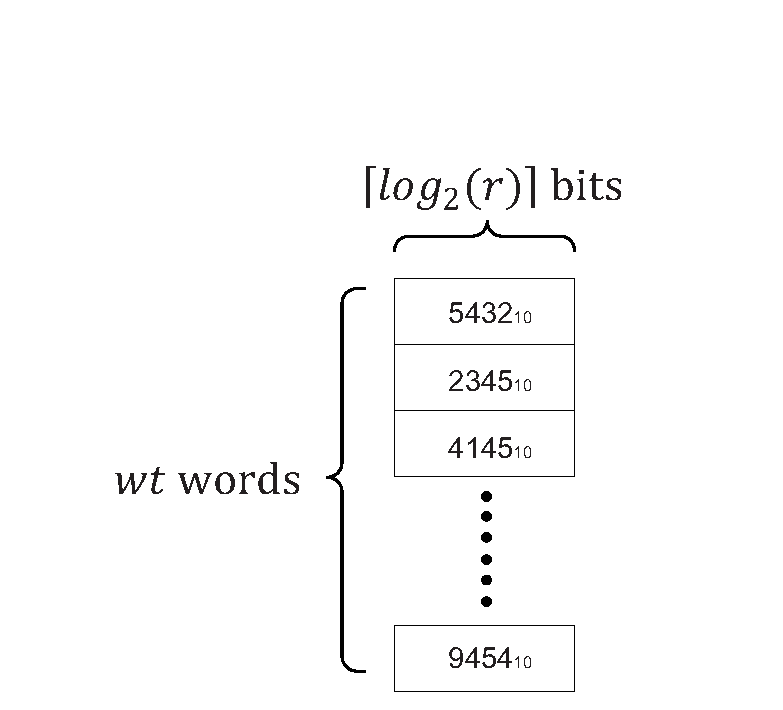
\includegraphics[width=\textwidth]{./fig/PolySparseFormat.eps}
\caption{Polynomial represented in sparse format}
\label{fig:poly_sparse}
\end{subfigure}
\caption{Polynomial in $\mathbb{F}_2[x]/(x^r+1)$ represented in different formats}
\label{fig::shifter}
\end{figure*}


\subsection{Polynomial Squaring}
\label{sub::square}
In this paper, the general squaring form $(a(x))^{2^n}$ is considered. The following theorem states how to calculate the squaring of a polynomial over $\mathcal{R}$.
\begin{theorem}
For squaring $(a(x))^{2^n}=\sum\widetilde{a_{i}}x^i$ of a polynomial $a(x)=\sum a_ix^i \in \mathcal{R}$, each coefficient $\widetilde{a_{i}}$ is updated by $a_{j}$ in $[{a_{r-1}},{a_{r-2}},\cdots,{a_0}]$ as:
\[
    \widetilde{a_{i}} = a_{i2^{-n}\bmod r}
\]
\end{theorem}

\begin{figure*}[!tb]
\centering
\begin{subfigure}[t]{0.5\textwidth}\centering
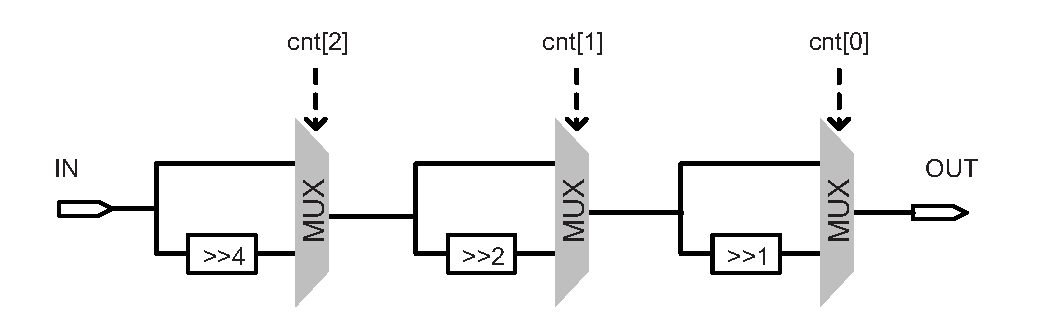
\includegraphics[width=\textwidth]{./fig/barrel1.eps}
\caption{Barrel shifter constructed by combinational logic}
\label{fig:barrel1}
\end{subfigure}
\hspace{1em}
\begin{subfigure}[t]{0.4\textwidth}\centering
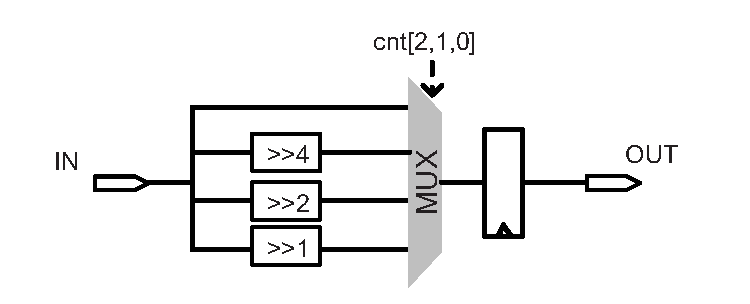
\includegraphics[width=\textwidth]{./fig/barrel2.eps}
\caption{Barrel shifter constructed by sequential logic}
\label{fig:barrel2}
\end{subfigure}
\caption{Barrel shifter used in our key generator to ensure constant execution of multiplication and squaring}
\end{figure*}

\begin{figure*}[!tb]
\centering
\begin{subfigure}[t]{0.45\textwidth}\centering
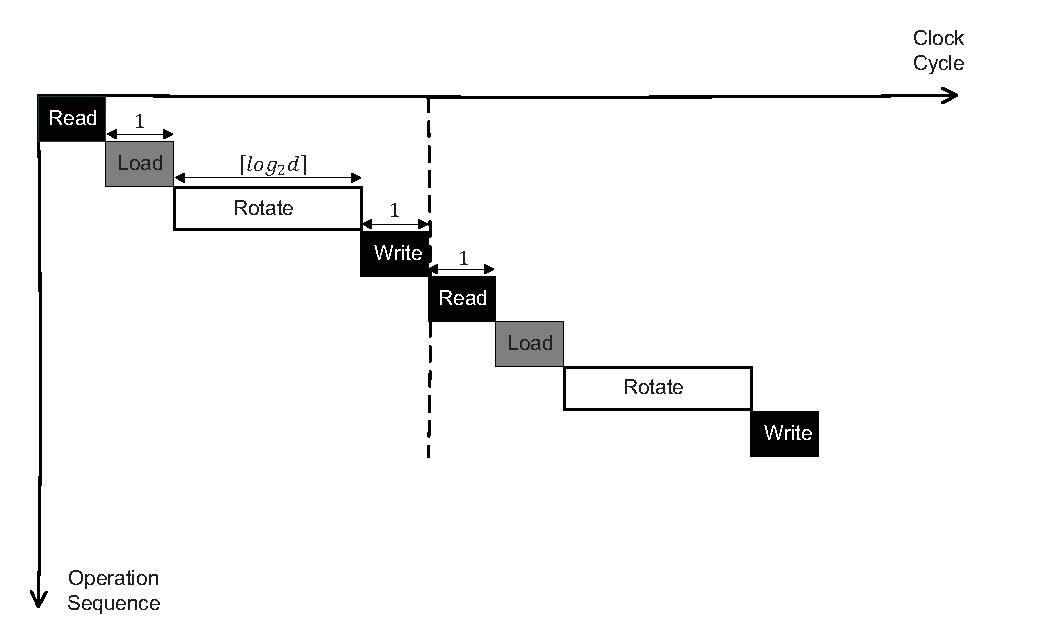
\includegraphics[width=\textwidth]{./fig/pipeline_square.eps}
\caption{Primitive operation pipelining for continuous square}
\label{fig:pipeline_squ}
\end{subfigure}
\hspace{1em}
\begin{subfigure}[t]{0.45\textwidth}\centering
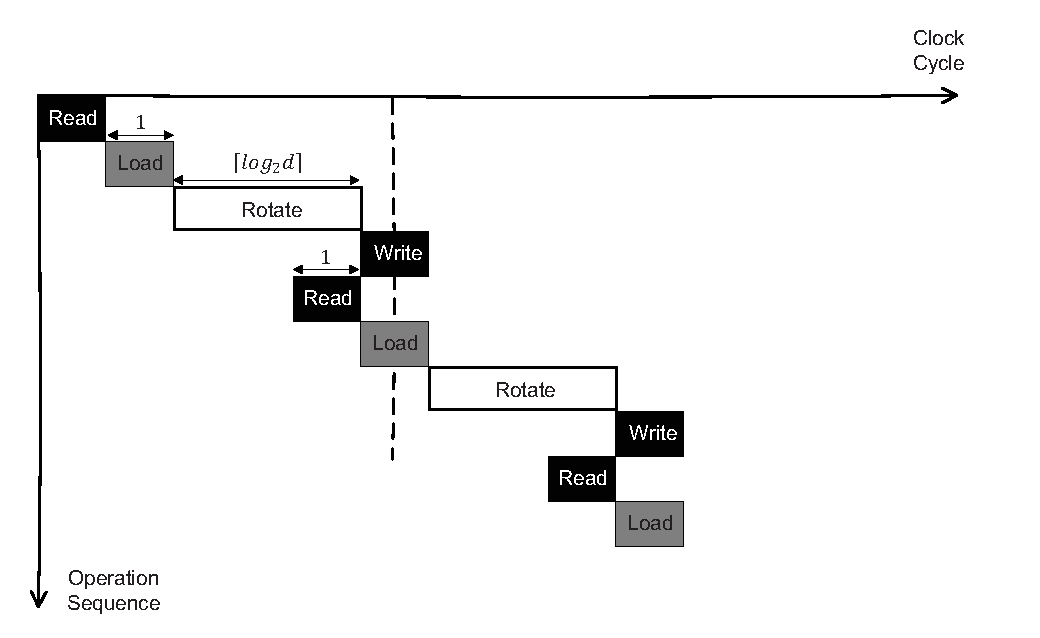
\includegraphics[width=\textwidth]{./fig/pipeline_square2.eps}
\caption{Optimised operation pipelining for continuous square }
\label{fig:pipeline_squ2}
\end{subfigure}
\caption{Timing diagram used in continuous square}
\end{figure*}

Note that the data is typically processed word by word on hardware, \textit{i.e.}, only one or two words (in our design, one word is $d$-bits) per time are fetched from memory and loaded to core function for further calculation. However, sometimes we want to extract the precise bit in the word.
Squaring is such an example where the result is indeed computed bit by bit.
To preserve the constant-time feature during executions while
avoiding the performance degradation in timing,
a Barrel shifter
is used to rotate the desired bit within $\lceil log_2d\rceil$ cycles. Barrel shifter can be built by pure combinational logic (shown in Fig.~\ref{fig:barrel1}) or sequential logic (shown in Fig.~\ref{fig:barrel2}). The sequential logic structure optimizes the critical path delay and is used in our design. By doing this, the computational steps for squaring $(a(x))^{2^n}$ are constant and independent of the value of $n$.

Figure~\ref{fig:pipeline_squ} depicts the pipeline stages for computing the
polynomial squaring operations continuously.
The basic computation pattern is:
First $a_{i2^{-n}}$ is read out from the memory,
then it gets loaded to the Barrel shifter and rotated to the correct bit position.
Finally the result is written back to the memory.
In general, such pattern repeats $r$ times and
hence the cycle count for computing the squaring operation continuously is:
$
r(\lceil log_2d\rceil+3)
$.

We further optimized the above pipeline based on the observation
that read and rotation operations can be parallelized,
and load and write can be parallelized as well,
the pipeline stages are shown in~\ref{fig:pipeline_squ}.
After this optimization, for computing the squaring operation continuously, we achieve a cycle count of:
$r(\lceil log_2d\rceil+1)+2$.


\subsection{Generic Polynomial Multiplication}
\label{sub::dense}
A generic polynomial multiplication involves two random dense polynomials.
For two dense polynomials $a(x)$ and $b(x)$, their multiplication is represented as:
\begin{align}
    a(x)\cdot b(x) &= (a_{r-1}x^{r-1}+\cdots + a_{1}x + a_0)\cdot(b_{r-1}x^{r-1}+\cdots + b_{1}x + b_0)\\
    &= \widetilde{c_{r-1}}x^{r-1}+\widetilde{c_{r-2}}x^{r-2}+\cdots + \widetilde{c_{1}}x +\widetilde{c_0}
\end{align}
%
For software implementations \cite{chou2016qcbits,drucker2017toolbox}, the best practice is to apply a carry-less Karatsuba algorithm to improve the performance for sufficiently high-degree polynomial multiplications, in particular those used for BIKE and other QC-MDPC code related cryptosystems. Carry-less Karatsuba algorithm is efficient on modern general-purpose processors equipped with ``carry-less multiplication'' instruction  PCLMULQDQ. This instruction computes the product of two binary polynomials of degree 63 and thus an appropriate software flow can use PCLMULQDQ to perform the carry-less Karatsuba algorithm for polynomials with any degree. However, FPGAs do not have
similar embedded instructions and moreover, a relatively complex control flow of Karatsuba algorithm will degrade the timing performance on FPGAs.
These issues drive us to find out a better solution for polynomial multiplications on FPGAs.


\begin{algorithm}[!tbh]
 \DontPrintSemicolon % Some LaTeX compilers require you to use \dontprintsemicolon instead
 \KwIn{dense polynomials $a(x),b(x) \in \mathbb{F}_2[x]/(x^r+1)$.}
 \KwOut{$a(x)\cdot b(x)\in \mathbb{F}_2[x]/(x^r+1)$}
    Reformulate $a(x)$ to block matrix view as $A[0],A[1],A[2],\ldots, A[n-1]$ where $n=\lceil r/d \rceil$, $d$ is the number of bits used in the row vector $A[i]$.\;
    Compute partial blocks from the transformation matrix $\text{BT}_{mul}$ associated with $b(x)$: $\text{BT}_{mul}[0,0]$, $\text{BT}_{mul}[0,1],\text{BT}_{mul}[0,2],\ldots,\text{BT}_{mul}[0,n-1]$ and $\text{BT}_{mul}[1,0]$, $\text{BT}_{mul}[2,0],\ldots,\text{BT}_{mul}[n-1,0]$\;
    The multiplication result is presented again in block matrix view $C[0],C[1],C[2],\ldots, C[n-1]$\;
    /*Diagonal Computation*/\;
    \For{$i \gets 0 \textbf{ to } n-1$}{
        $C[i] \gets A[i]\cdot \text{BT}_{mul}[0,0]$\;
    }
    /*Upper Triangle Computation*/\;
    \For{$i \gets 1 \textbf{ to } n-1$}{
        \For{$j \gets 0 \textbf{ to } n-1-i$}{
           $C[i+j] \gets C[i+j] + A[j]\cdot \text{BT}_{mul}[0,i]$\;
        }
    }
    /*Lower Triangle Computation*/\;
    \For{$i \gets 1 \textbf{ to } n-1$}{
        \For{$j \gets 0 \textbf{ to } n-1-i$}{
           $C[j] \gets C[j] + A[i+j]\cdot \text{BT}_{mul}[i,0]$\;
        }
    }
    \Return {the vector $C=[C[0],C[1],\ldots,C[n-1]]$ as the coefficients of $c(x)=a(x)b(x)$\;}
 \caption{Proposed generic multiplication algorithm}\label{alg:generic_mul}
\end{algorithm}

A formal description of the proposed generic multiplication algorithm
can be found in Algorithm~\ref{alg:generic_mul}.
As we can see, this algorithm is computed in exactly $n^2$ steps with $n=\lceil r/d\rceil$, and therefore, for fixed BIKE parameters $r$ and $d$, the computational time is also fixed.
The core function in the generic polynomial multiplication
is the multiplication of a $d$-bit vector $A[k]$ of $a(x)$ and a block matrix $\text{BT}_{mul}$$[i,j]$ from $\text{BT}_{mul}$:
\[
    [a_j,a_{j+1},\ldots,a_{j+d-1}]\cdot
\left[ \begin{array}{ccccc}
b_{i}&b_{i+1}&b_{i+2}&\cdots &b_{i+d-1} \\
b_{i-1}&b_{i}&b_{i+1}&\cdots &b_{i+d-2} \\
\vdots&\vdots&\vdots&\vdots&\vdots\\
b_{i-d+1}&b_{i-d+2}&b_{i-d+3}&\cdots &b_{i} \\
\end{array}
\right ]_{d\times d}
\]
We design a dedicate hardware core for the above multiplication which can be
finished in one clock cycle, as depicted in Figure~\ref{fig:gmul_core}.
With this module, the proposed generic multiplication algorithm
can be scheduled as shown in Figure~\ref{fig:pipeline_gmul}.
Read takes 5 cycles to balance the critical path for reading $B[i,j]$.
A dual-port RAM is used such that the target vector $B[i,j]$ can be loaded within two cycles. Here a fixed rotation is performed to move $A[k]$ to the correct bit positions.
The MUL module performs the core multiplication $A[k]\cdot B[i,j]$ and later writes
the result back.




%\begin{table}[!tb]\centering
%\caption{Cycle counts for computing one block in Generic Multiplication}
%\begin{tabular}{c|c|c|c}
%  \hline
%  % after \\: \hline or \cline{col1-col2} \cline{col3-col4} ...
%  Operation & Load & Rotate & Mul  \\\hline
%   & 5 & 2 & 1  \\
%  \hline
%\end{tabular}
%\end{table}



\begin{figure*}[!tb]
\centering
\begin{subfigure}[t]{0.47\textwidth}\centering
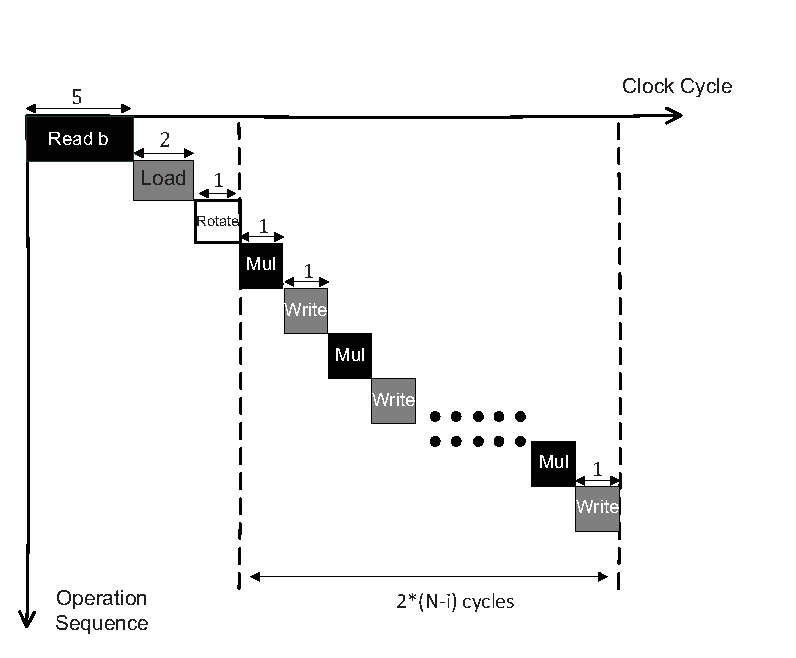
\includegraphics[width=\textwidth]{./fig/pipeline_dsnmul.eps}
\caption{Primitive operation pipelining for generic multiplication}
\label{fig:pipeline_gmul}
\end{subfigure}
\hspace{1em}
\begin{subfigure}[t]{0.47\textwidth}\centering
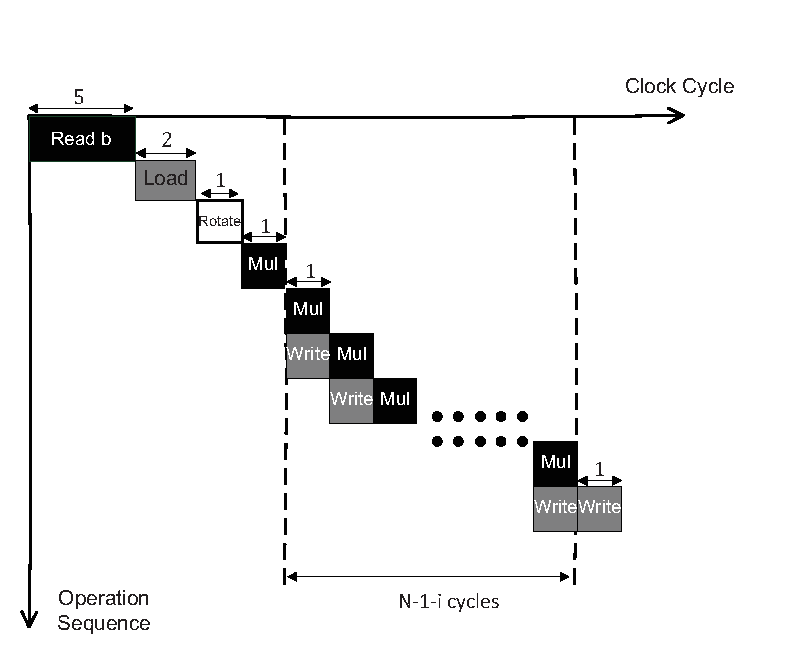
\includegraphics[width=\textwidth]{./fig/pipeline_dsnmul2.eps}
\caption{Optimised operation pipelining for generic multiplication }
\label{fig:pipeline_gmul2}
\end{subfigure}
\caption{Timing diagram used in generic multiplication}
\end{figure*}


\begin{figure}[!tb]
\centering
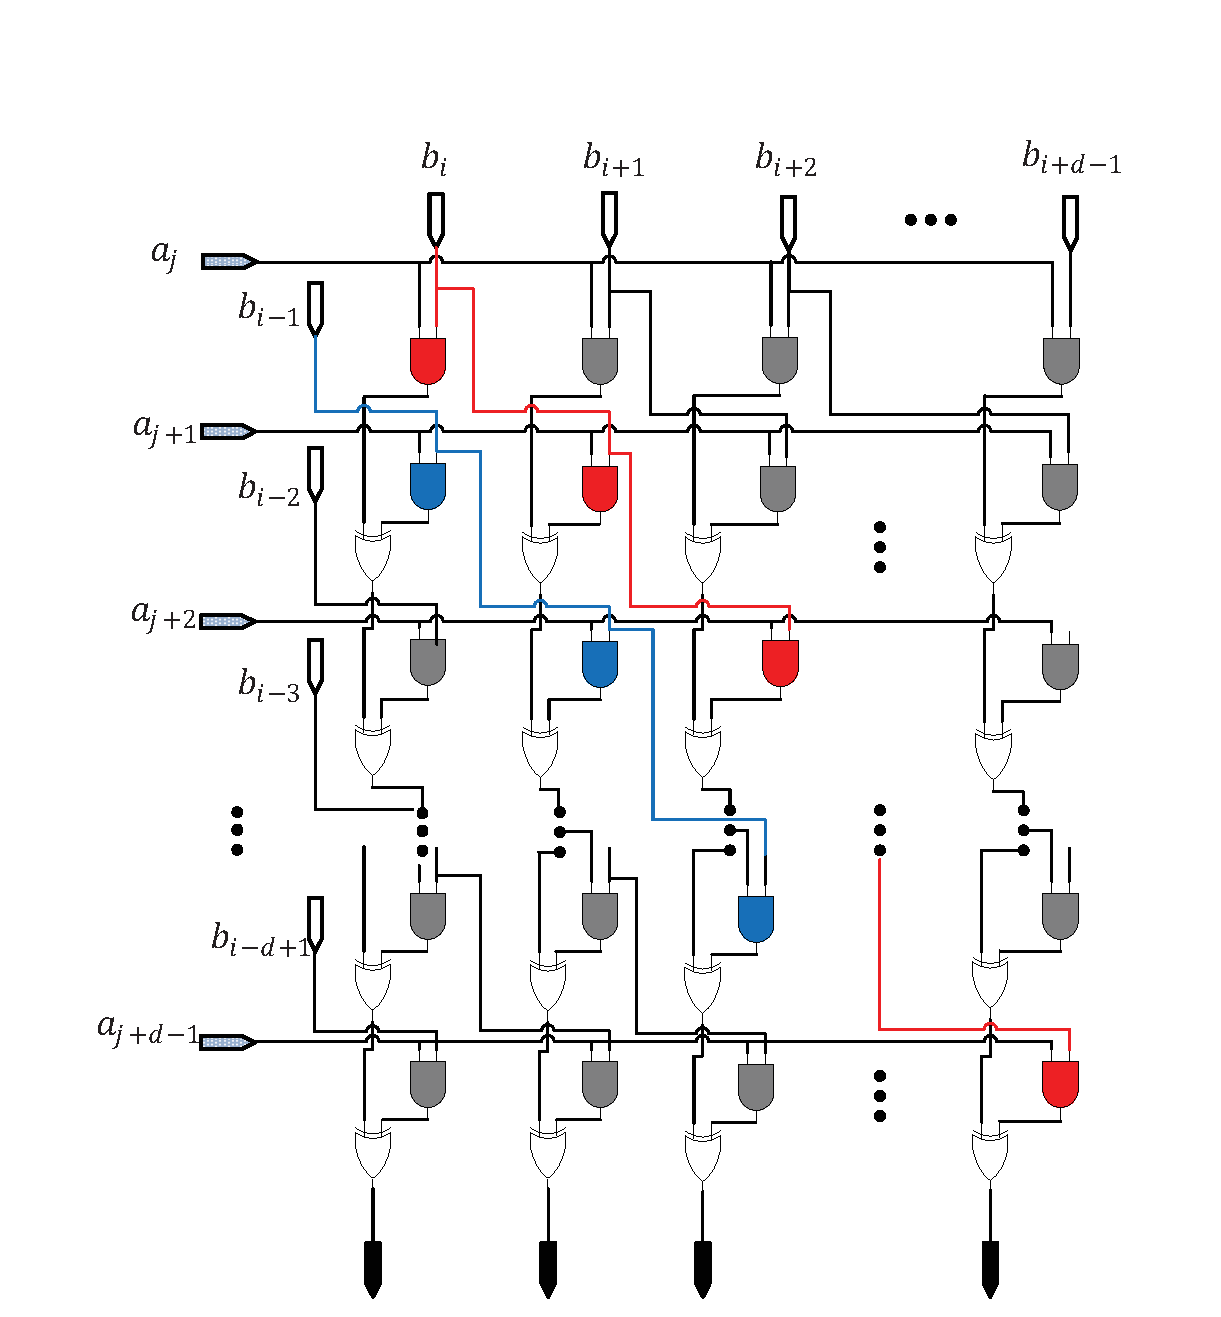
\includegraphics[width=.55\textwidth]{./fig/dsnmul_core.eps}
\caption{Architectural overview of the core unit in the generic multiplication}\label{fig:gmul_core}
\end{figure}


An improved schedule is depicted in Figure~\ref{fig:pipeline_gmul2}
where Mul and Write perform simultaneously.
To handle the diagonal computation,
it takes $5+2+1+2\lceil r/d\rceil$ cycle count where $i=0$. $\lceil r/d\rceil -1$ iterations are required for the upper triangle computation.
For the $i=1,2,\ldots,d-1$-th iteration, it
consumes $5+2+1+\lceil r/d\rceil -1-i+1$ cycles.
Therefore the entire upper triangle computation costs $(\lceil r/d\rceil^2 +17\lceil r/d\rceil-18)/2$ cycles.
The same cycle count is needed for the lower triangle computation.

In general, the cycle count for the optimised generic polynomial multiplication is:
$\lceil r/d\rceil^2 + 18\lceil r/d\rceil - 9$.



\subsection{Sparse Polynomial Multiplication}
\label{sub::sparse}
In BIKE, a special form of multiplication called sparse polynomial multiplication,
is frequently used. In sparse polynomial multiplication, one of the operands
is a sparse polynomial whereas the other one is a dense polynomial.
Such multiplications can be efficiently computed as follows:
The sparse polynomial, \textit{e.g}, $a(x)$ is first represented
by an array of indices in $I=\{i|a_i=1\}$.
Then, the multiplication result can be obtained by extracting $i\in I$ rows of $\text{BT}_{mul}$ and then accumulating them, \textit{i.e.}, $\sum_{i\in I} x^ib(x)$ and the $i$-th row of the matrix $\text{BT}_{mul}$ represents the coefficients of $x^ib(x)$. Formally, the coefficient vector of sparse polynomial multiplication can be calculated as:
$\sum_{i\in I} [b_{-i},b_{-i+1},\cdots,b_{-i-1}]$.

%\begin{table}[!tb]\centering
%\caption{Cycle counts for extracting $d$ bits of $x^ib(x)$ in Sparse Polynomial Multiplication{\color{red} you did not mention this table anywhere in the text}}
%\begin{tabular}{c|c|c|c|c|c|c|c}
%  \hline
%  % after \\: \hline or \cline{col1-col2} \cline{col3-col4} ...
%  Operation & Read\_h & Read\_g & Load &Rotation & Add & Write & Total \\\hline
%   & 3 & 3 & 2 & $\lceil log_2(d)\rceil$ & 1 & 1& 10+$\lceil log_2(d)\rceil$ \\
%  \hline
%\end{tabular}
%\end{table}

% \begin{figure*}[!tb]
% \centering
% \begin{subfigure}[t]{0.5\textwidth}\centering
% 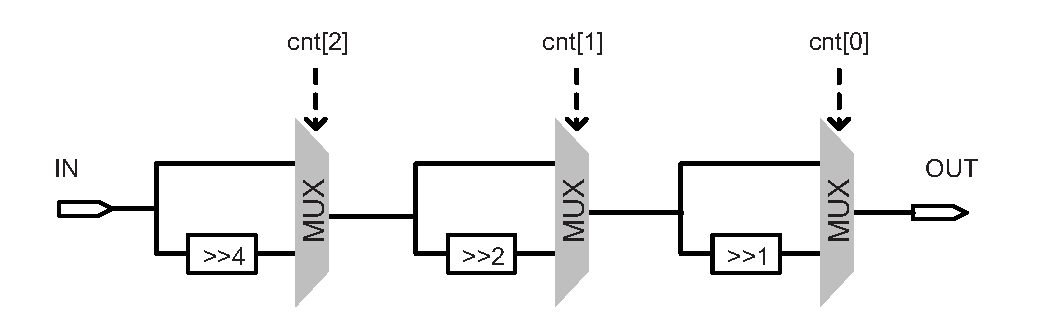
\includegraphics[width=\textwidth]{./fig/barrel1.eps}
% \caption{Barrel shifter constructed by combinational logic}
% \label{fig:L1_ctrl}
% \end{subfigure}
% \hspace{1em}
% \begin{subfigure}[t]{0.4\textwidth}\centering
% 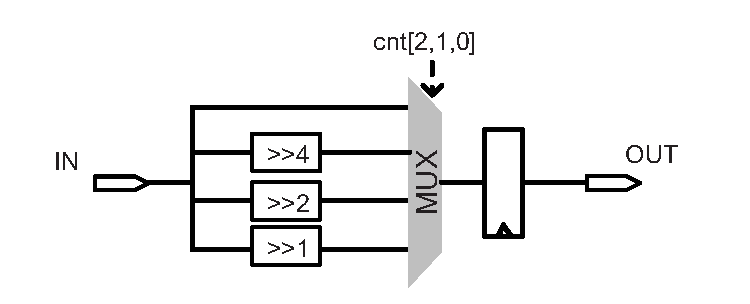
\includegraphics[width=\textwidth]{./fig/barrel2.eps}
% \caption{Barrel shifter constructed by sequential logic}
% \label{fig:FLIP_ctrl}
% \end{subfigure}
% \caption{Barrel shifter used in our key generator to ensure constant execution of multiplication and squaring}
% \end{figure*}





\begin{figure*}[!tb]
\centering
\begin{subfigure}[t]{0.47\textwidth}\centering
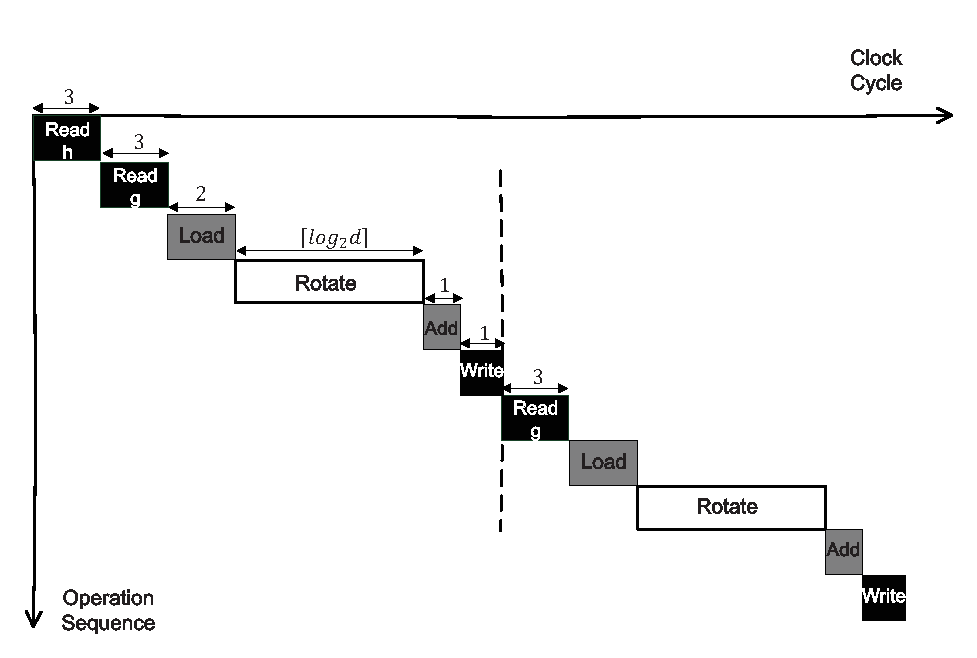
\includegraphics[width=\textwidth]{./fig/pipeline_mul.eps}
\caption{Primitive operation pipelining for sparse polynomial multiplication}
\label{fig:pipeline_mul}
\end{subfigure}
\hspace{1em}
\begin{subfigure}[t]{0.47\textwidth}\centering
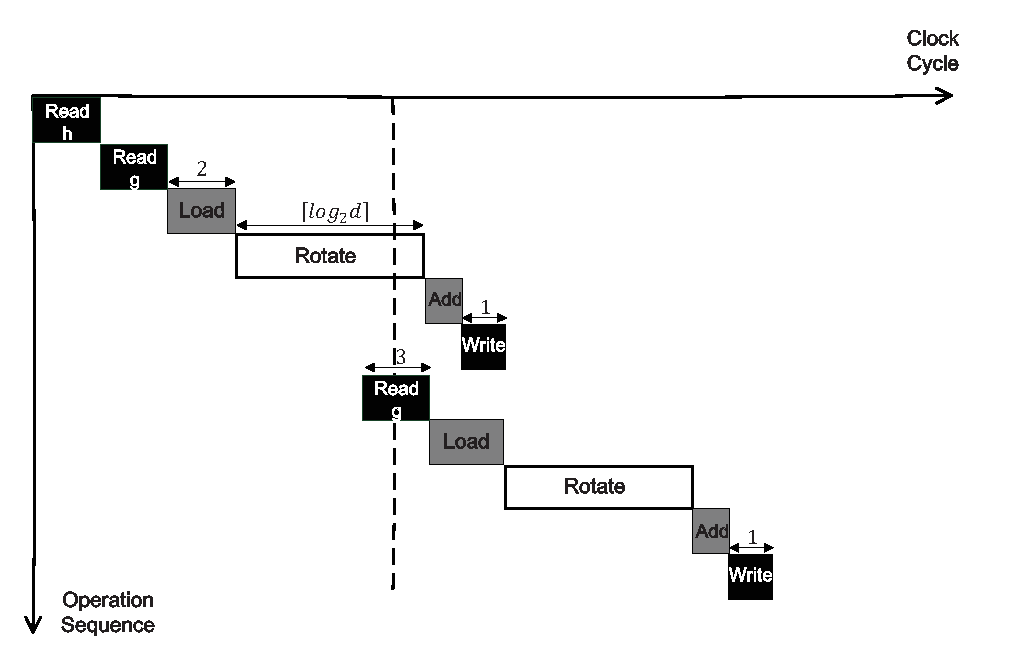
\includegraphics[width=\textwidth]{./fig/pipeline_mul2.eps}
\caption{Optimised operation pipelining for sparse polynomial multiplication }
\label{fig:pipeline_mul2}
\end{subfigure}
\caption{Timing diagram used in sparse polynomial multiplication}
\end{figure*}

\begin{table}[!tb]\centering
\caption{Cycle count comparison between unoptimized and optimized sparse polynomial multiplication. The pipelined architecture introduces about 50\% reduction of cycle count for all BIKE instances}
\begin{tabular}{cc|ccccc}
  \hline
  % after \\: \hline or \cline{col1-col2} \cline{col3-col4} ...
 \textbf{Category}        &             & $d$ & $r$  & $|I|=w/2$  & unoptimized version& optimized version\\\hline
\multirow{ 2}{*}{128-bit} &  BIKE-[1,2] & $64$ & $10163$  & $71$  & $180,624$ & $90,880$\\
                          &  BIKE-[3] & $64$ & $11027$  & $67$  & $185,456$& $93,264$\\
  \hline
\multirow{ 2}{*}{192-bit} &  BIKE-[1,2] & $64$ & $19853$  & $103$  &$512,528$& $257,088$\\
                          &  BIKE-[3] & $64$ & $21683$  & $99$  &$536,976$& $269,280$\\
  \hline
\multirow{ 2}{*}{256-bit} &  BIKE-[1,2] & $64$ & $32749$  & $137$  &$1,122,304$& $562,248$\\
                          &  BIKE-[3] & $64$ & $36131$  & $133$  &$2,404,640$& $1,203,384$\\
  \hline
\end{tabular}
\label{tab::sparse}
\vspace{-4mm}
\end{table}

Figure~\ref{fig:pipeline_mul} depicts the basic pipeline schedule where the total cycle count for one complete sparse polynomial multiplication is:
$|I|\cdot\lceil r/d\rceil\cdot (10+\lceil log_2(d)\rceil)$.

The cycle count can be further improved if Read\_g is computed in parallel
with Rotate while Load is computed in parallel with Add+Write.
This optimized schedule for pipelining is presented in Figure~\ref{fig:pipeline_mul2}
and the optimized cycle count is:
$
|I|(\lceil r/d\rceil\cdot (2+\lceil log_2(d)\rceil) + 8)
$.

Table~\ref{tab::sparse} present the cycle count
of the two pipeline scheduling schemes. The optimized pipeline can improve the cycle count by about 50\%.

\subsection{Polynomial Inversion}
\label{sub::inversion}
\begin{theorem}
Let $a$ be an invertible polynomial in the quotient ring $\mathbb{F}_2[x]/(x^r+1)$ where $r$ is a prime, then the inverse of polynomial $a$ can be computed as $a^{-1}=(a^{2^{r-2}-1})^2$
\end{theorem}
%
According to Theorem~1, we can compute the inverse of a
polynomial over ring $\mathbb{F}_2[x]/(x^r+1)$
by exponentiation.
To efficiently compute the exponentiation of the polynomial,
we propose a method which is described as follows.
First, we define a function $\beta_{k}(a)=a^{2^k-1}$.
It is easy to see that $a^{-1}=(\beta_{r-2}(a))^2$. % in the quotient ring $\mathbb{F}_2[x]/(x^r+1)$.
Therefore, this recursive
formula holds:
$\beta_{k+j}(a)=(\beta_{k}(a))^{2^j}\beta_{j}(a)$.
%
\begin{algorithm}[!tb]
\DontPrintSemicolon % Some LaTeX compilers require you to use \dontprintsemicolon instead
\KwIn{$r-2=(r_{q-1} \ldots r_0)_2$ and $\alpha \in \mathbb{F}_2[x]/(x^r+1)$.}
\KwOut{$\beta =  \alpha ^{-1}$}
$\beta \gets \alpha$ \;
$t \gets 1$ \;
\For{$i \gets q-2$ \textbf{to} $0$}{
    $\beta \gets (\beta )^{2^{t}} \cdot \beta$\;
    $t \gets 2t$\;
   \uIf{$r_i = 1$}{
        $\beta \gets (\beta)^{2} \cdot  \alpha $\;
        $t \gets t + 1$\;
    }
}
 $\beta \gets \beta ^2$ \;
\Return {$\beta$}


\caption{Itoh-Tsujii Inversion Algorithm (ITA) \cite{hu2015fast}}
\label{algo:ITA}
\end{algorithm}



% \subsection{Polynomial Arithmetics}
\begin{figure}[!tb]
\centering
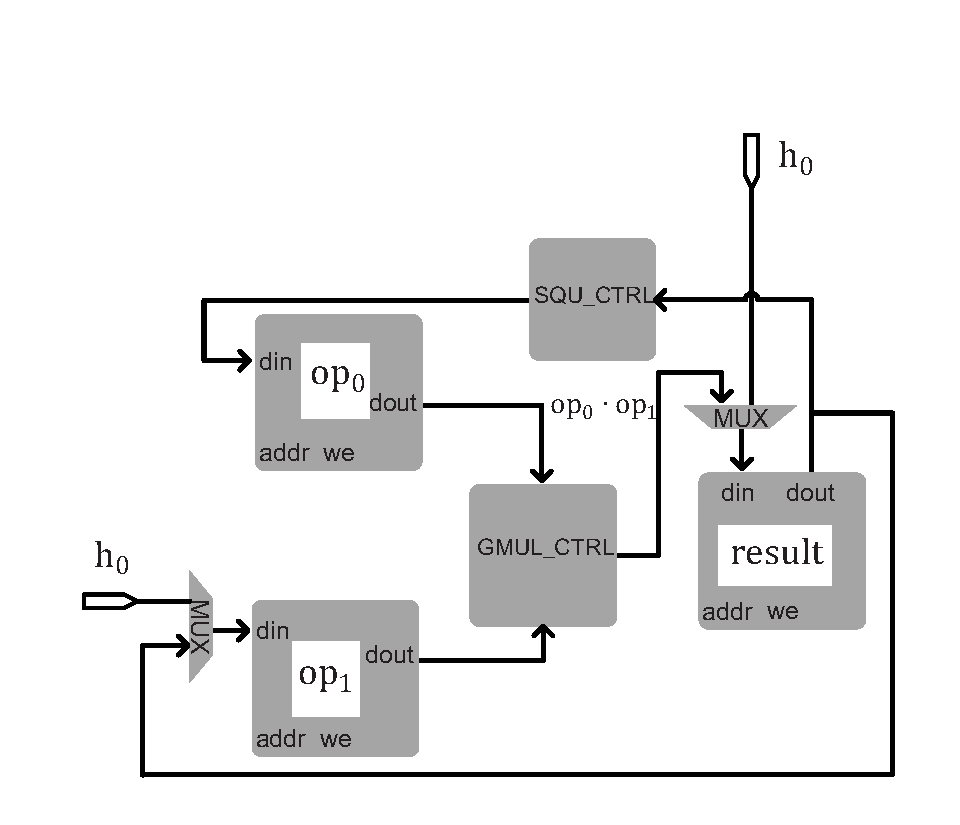
\includegraphics[width=.55\textwidth]{./fig/inv_unit.eps}
\caption{Diagram of the polynomial inversion architecture}\label{fig:inverter}
\end{figure}
With the above recursion formula, we can generate $\beta_{r-2}(a)$ from $\beta_{1}(a)=a$
through an addition chain in constant steps, which is known as
Itoh-Tsujii Inversion algorithm (ITA), as shown in Algorithm~\ref{algo:ITA}.
More importantly, the building blocks for ITA are
polynomial squaring and multiplication which
can be highly optimized in our design.
Another common approach for polynomial inversion
is through the Extended Euclidean algorithm (EEA).
In \cite{georgieva2015toward}, EEA with constant flow is
proposed which can be exploited for secure polynomial inversions.
However, the steps in the proposed algorithm are data-dependent
and thus is not suitable for parallel designs on hardware.
% In summary, we implement the algorithmic description for ITA from \cite{hu2015fast} as shown in Algorithm.
An illustrative example for computing the polynomial inversion used in
BIKE-2 is shown in Table~\ref{table:ita_example} in the Appendix.

% From this table, we can see that ITA is not only efficient
% (20 multiplications + 20 squarings)
By use of ITA, the polynomial inversion operation
can be performed in constant time.
Figure~\ref{fig:inverter} depicts the diagram of the ITA inverter.
The input polynomial $\alpha$ is used to initialize the RAM result.
Then the polynomial $\beta$ stored in the RAM is raised
to ${\beta}^{2^t}$ by use of the SQU\_CTRL module which
is the module for polynomial squaring as described
in Section~\ref{sub::square}.
The result is then stored to RAM op0.
The GMUL\_CTRL module (Section~\ref{sub::dense}) performs a
generic polynomial multiplication
(step 4,7, Algorithm~\ref{algo:ITA}).
After the final squaring operations (step 10),
the inverted polynomial is stored as the result in RAM op0.
% In the following subsections,
% we detail the squaring and the generic multiplication used in ITA.



\subsection{Generation of Polynomials with Prescribed Weight}\label{sub::polygen}

\begin{algorithm}[!tb]
\DontPrintSemicolon % Some LaTeX compilers require you to use \dontprintsemicolon instead
\KwIn{PRNG seed, polynomial length $r$, data width $d$}
\KwOut{binary vector $\mathbf{ \overline{f}}$ representing $f=f_0+\ldots +f_{r-1}x^{r-1}\in \mathbb{F}_2[x]/(x^r+1)$, with odd weight $|f|\approx r/2$}
$wt \gets 0$\;
\For{$i \gets 0 \textbf{ to } \lceil r/d\rceil-1$}{
    $\overline{\mathbf{f}[i]} \gets \text{truncate}_{d}(SecureRand(seed))$\;
    $wt \gets wt+|\overline{\mathbf{f}[i]}|$
}
\uIf{$wt$ is even}{
        flip the first bit in $\overline{\mathbf{f}[i]}$
	  }
\Return {$\overline{\mathbf{f}}$}


\caption{Generation of a random polynomial with odd weight}
\label{alg:prng1}
\end{algorithm}

\SetKwRepeat{Do}{do}{while}%
\begin{algorithm}[!tb]
\DontPrintSemicolon % Some LaTeX compilers require you to use \dontprintsemicolon instead
\KwIn{PRNG seed, polynomial length $r$, data width $d$, polynomial weight $wt=w/2$}
\KwOut{ integer vector $\mathbf{ \hat{f}}$ contains non-zero bit-positions ($\{i|f_i\neq 0\}$  to represent $f=f_0+\ldots +f_{r-1}x^{r-1}\in \mathbb{F}_2[x]/(x^r+1)$, with odd weight $|f|= wt$}
\For{$i \gets 0 \textbf{ to } wt-1$}{
    \Do{$rand \geq r$ or  $rand \in \mathbf{\hat{f}}$ }{
      $rand \gets \text{truncate}_{d}(SecureRand(seed))$\;
    }
    $\mathbf{ \hat{f}}[i] \gets rand$
}
\Return {$\mathbf{ \hat{f}}$}


\caption{Generation of a random sparse polynomial with given (odd) weight}
\label{alg:prng2}
\end{algorithm}

Strictly speaking, the execution time of the random polynomial generations proposed in
Algorithms~\ref{alg:prng1}, \ref{alg:prng2} is non-constant.
Algorithm~\ref{alg:prng1} optionally performs a step if the
Hamming weight of the polynomial is an even number;
Algorithm~\ref{alg:prng2} keeps generating new random numbers
until a non-repeated number smaller than the system parameter $r$
is generated.
Nevertheless, in the following text we validate that
these non-constant-time behaviors do not leak any secret
information that can be exploited by an adversary:
The optional step in Algorithm~\ref{alg:prng1}
flips the first bit-position of $\mathbf{\overline{f}}$
and the probabilistic distribution of this bit position
does not change as long as the PRNG itself is unbiased (uniformly distributed).
An adversary has no advantage in estimating the value
of this specific bit even if he observes the timing difference.
For Algorithm~\ref{alg:prng2}, the timing difference
observed by an adversary is actually the total amount
of time introduced by the re-generation of random numbers
when an overflow ($rand\geq r$) or a repetition ($rand\in \mathbf{\hat{f}}$) occurs.
An overflow does not leak any information about $\mathbf{\hat{f}}$
as the information that the generated number is above $r$ does
not leak any information on $\mathbf{\hat{f}}$.
The probability that the generated random number is smaller
than $r$ is $Pr(\text{rand} < r)= r/2^{\lceil log_2(r)\rceil}$.
To eliminate the possible timing leakage from the repetition,
we introduce a method by changing the while-loop
in step 4 of Alg.~\ref{alg:prng2} to while $rand\geq r$.
In another word, we generate $w_t$ random numbers each
of which is smaller than $r$ without considering whether they collide
with each other or not.
By doing this, no timing information is leaked on repetition but
in this case, a few repetitions might occur which in turn reduces
the Hamming weight of the generated sparse polynomial.
However, a small loss of Hamming weight $w$ is tolerable in BIKE:
% is not sensitive to a slight loss of Hamming weight $w$.
To reach $\lambda$ bits of classical security, $\lambda\approx w-log_2r$ for
BIKE-1 and BIKE-2 and $\lambda\approx w-\frac{1}{2}log_2r$ for BIKE-3,
and 1 or 2 repetitions only decrease the security from $2^\lambda$ to $2^{\lambda-2}$.
More importantly, the probability that a single run of Algorithm~\ref{alg:prng2} without considering collision succeeds if we tolerate one or two repetitions:
\begin{align}
    %Pr(\text{Alg.~\ref{alg:prng2} succeeds}) &=
    Pr(\text{Alg.~\ref{alg:prng2} succeeds})
    &=\frac{r(r-1)\cdots (r-w_t+1)}{r^{w_t}}+ \frac{\binom{w_t}{2}r(r-1)\cdots (r-w_t+2)}{r^{w_t}}\\
    &+ \frac{[\binom{w_t}{3}+\binom{w_t}{2}\binom{w_t-2}{2}/2]  r(r-1)\cdots (r-w_t+3) }{r^{w_t}}
\end{align}
The probability is very high (at least 0.997, as shown in Table~\ref{table:success_rate}):


% \begin{figure*}[!tb]
% \centering
% \begin{subfigure}[t]{0.45\textwidth}\centering
% 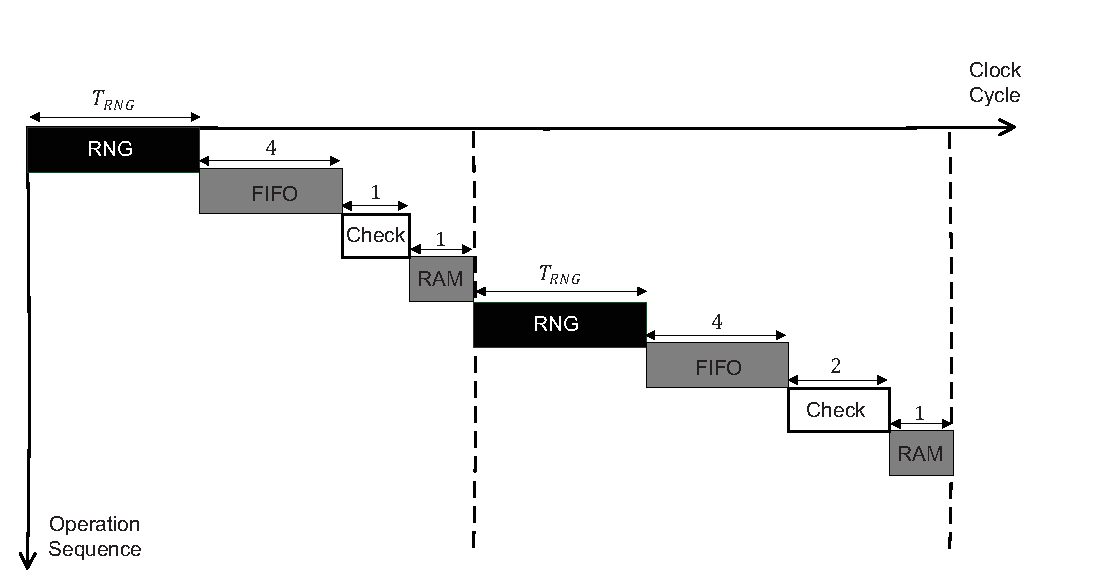
\includegraphics[width=\textwidth]{./fig/pipeline_rng.eps}
% \caption{Primitive operation pipelining for Algorithm~\ref{alg:prng2}}
% \label{fig:pipeline_rng}
% \end{subfigure}
% \hspace{1em}
% \begin{subfigure}[t]{0.45\textwidth}\centering
% 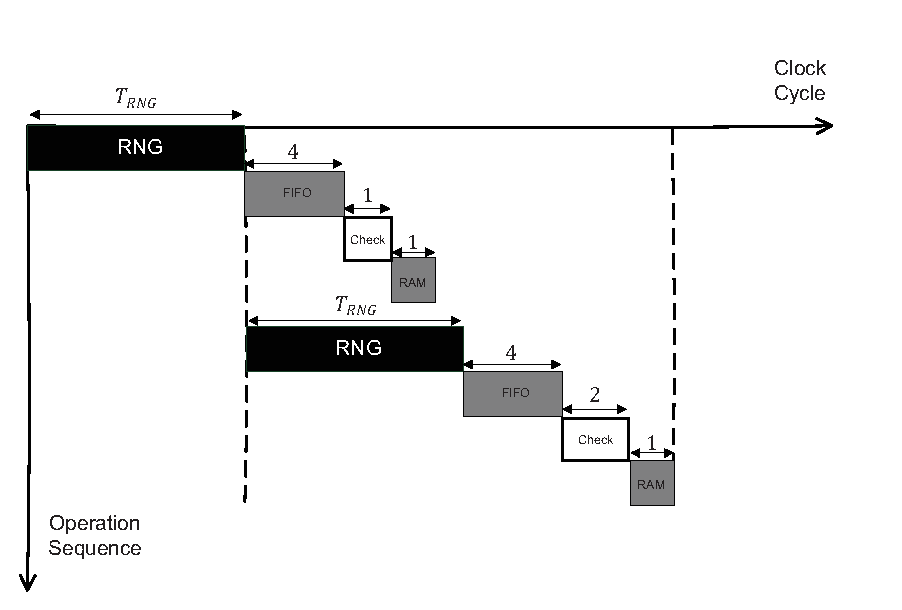
\includegraphics[width=\textwidth]{./fig/pipeline_rng2.eps}
% \caption{Optimised operation pipelining for Algorithm~\ref{alg:prng2} (initial phase) }
% \label{fig:pipeline_rng2}
% \end{subfigure}
% \begin{subfigure}[t]{0.45\textwidth}\centering
% 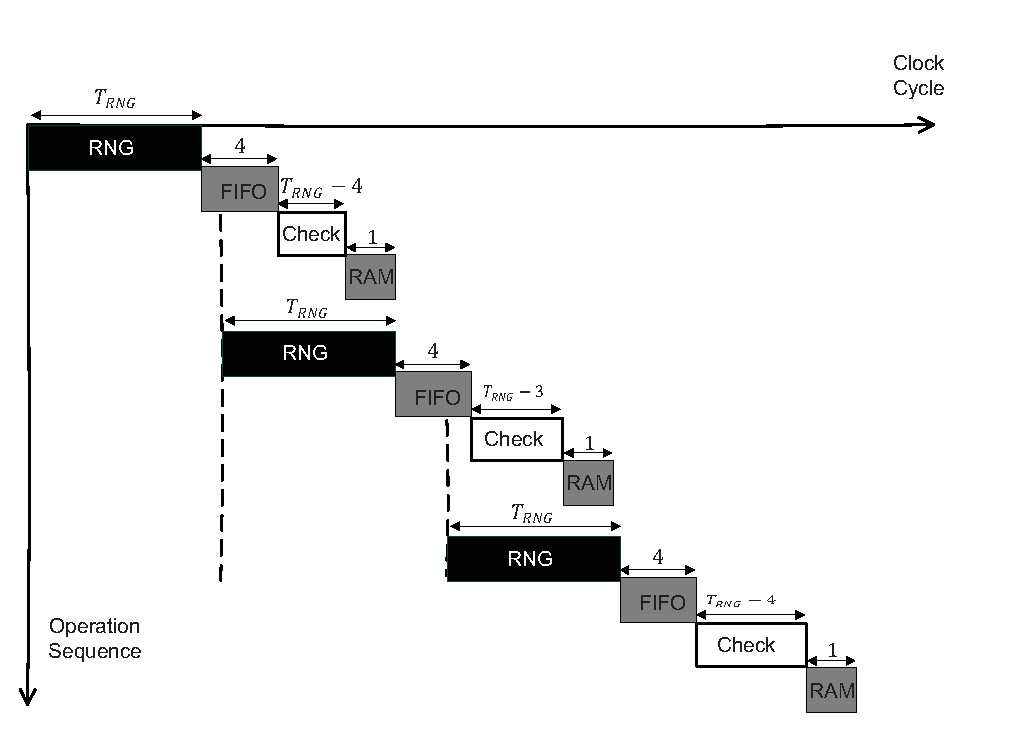
\includegraphics[width=\textwidth]{./fig/pipeline_rng3.eps}
% \caption{Optimised operation pipelining for Algorithm~\ref{alg:prng2} (final phase) }
% \label{fig:pipeline_rng3}
% \end{subfigure}
% \caption{Timing diagram used for generating a random polynomial with odd weight}
% \end{figure*}

\begin{table}[!tb]\centering
\caption{Success Rate for generating a random polynomial with odd weight using Algorithm~\ref{alg:prng2}}\label{table:success_rate}
\begin{tabular}{cc|cccc}
  \hline
  % after \\: \hline or \cline{col1-col2} \cline{col3-col4} ...
 \textbf{Category}        &             & no repetition & 1 repetition & 2 repetitions & success rate \\\hline
\multirow{ 2}{*}{128-bit} &  BIKE-[1,2] & $0.7826$ & $0.1926$  & $0.0228$  & $0.9981$\\
                    &  BIKE-[3] & $0.8179$ & $0.1649$  & $0.0159$  & $0.9989$\\
  \hline
\multirow{ 2}{*}{192-bit} &  BIKE-[1,2] & $0.7671$ & $0.2040$  & $0.0264$  & $0.9976$\\
                    &  BIKE-[3] & $0.7992$ & $0.1796$  & $0.0196$  & $0.9985$\\
  \hline
\multirow{ 2}{*}{256-bit} &  BIKE-[1,2] & $0.7521$ & $0.2148$  & $0.0300$  & $0.9970$\\
                    &  BIKE-[3] & $0.7840$ & $0.1911$  & $0.0228$  & $0.9981$\\
  \hline
\end{tabular}
\vspace{-4mm}
\end{table}



%Now assume $t$ (typically small compared with $wt$) repetitions happen after a single run of Algorithm~\ref{alg:prng2}. The number of possible $t$ repetitions within $wt+t$ times of random number generations is:
%\[
%    \frac{r!}{(r-wt)!} \cdot wt^t
%\]
%For typical system parameters in BIKE and LEDA, this number is too large (\textit{e.g.}, $\geq 2^{944}$ in BIKE-1 settings with 128-bit SL) which is beyond computational capacity to analyze.

Note that the design uses a simple PRNG based on linear congruence to enable deterministic generation of random numbers (\textit{i.e.}, the function of $SecureRand(\cdot)$ in Algorithm~\ref{alg:prng1}, \ref{alg:prng2}). For real-world deployment,
such PRNG must be replaced with a cryptographically secure random number
generator, \textit{e.g.}, \cite{laue2007compact,cherkaoui2013very}. We require at most $d$ random bits per $T_{\text{PRNG}}$ clock cycles where $T_{\text{PRNG}}=13$ in our settings.
The average clock cycles for generating a qualified rand number is $T_{\text{PRNG}}' = T_{\text{PRNG}}/Pr(\text{rand} < r)$

%\begin{table}[!tb]\centering
%\caption{Cycle counts for generating  one entry of a random polynomial with odd weight}
%\begin{tabular}{c|c|c|c}
%  \hline
%  % after \\: \hline or \cline{col1-col2} \cline{col3-col4} ...
%  Operation & PRNG & Write & Total \\\hline
%   & $T_{\text{PRNG}}$ & 1  & $T_{\text{PRNG}}$+1 \\
%  \hline
%\end{tabular}
%\vspace{-4mm}
%\end{table}
%
%\begin{table}[!tb]\centering
%\caption{Cycle counts for generating  the i-th entry (i=1,2,...) of a random sparse polynomial with odd weight}
%\begin{tabular}{c|c|c|c|c|c}
%  \hline
%  % after \\: \hline or \cline{col1-col2} \cline{col3-col4} ...
%  Operation & PRNG & Rd\_FIFO & CHECK &Wr\_RAM & Total \\\hline
%   & $T_{\text{PRNG}}$ & 4  & $i$ & 1 &$T_{\text{PRNG}}+5+i$ \\
%  \hline
%\end{tabular}
%\vspace{-4mm}
%\end{table}

\begin{table}[!tb]\centering
\caption{Cycle counts for generating the sparse polynomial $h_0/h_1$ in BIKE KeyGen}\label{table:spare_ploy_gen}
\begin{tabular}{cc|ccccc}
  \hline
  % after \\: \hline or \cline{col1-col2} \cline{col3-col4} ...
 \textbf{Category}        &             & Total & $r$  & $w_t$  & $Pr(\text{rand} < r)$& $Pr(\text{Alg.~\ref{alg:prng2} succeeds})$\\\hline
\multirow{ 2}{*}{128-bit} &  BIKE-[1,2] & $1279$ & $10163$  & $71$  & $0.62$ & $0.9981$\\
                          &  BIKE-[3] & $1062$ & $11027$  & $67$  & $0.67$& $0.9989$\\
  \hline
\multirow{ 2}{*}{192-bit} &  BIKE-[1,2] & $2120$ & $19853$  & $103$  &$0.60$& $0.9976$\\
                          &  BIKE-[3] & $1847$ & $21683$  & $99$  &$0.66$& $0.9985$\\
  \hline
\multirow{ 2}{*}{256-bit} &  BIKE-[1,2] & $2801$ & $32749$  & $137$  &$0.99$& $0.9970$\\
                          &  BIKE-[3] & $3350$ & $36131$  & $133$  &$0.55$& $0.9981$\\
  \hline
\end{tabular}
\vspace{-4mm}
\end{table}

Therefore, the total cycle count for generating a random polynomial with odd weight (Algorithm~\ref{alg:prng1}) is
$\lceil r/d\rceil\cdot T_{\text{PRNG}} + 1$.


We use the average case for Algorithm~\ref{alg:prng2} to estimate the clock cycle count for generating a random sparse polynomial with given (odd) weight:
\[
   \left(w_tT'_{\text{PRNG}} + \frac{w_t(w_t+1)}{2} + 5w_t\right)/Pr(\text{Alg.~\ref{alg:prng2} succeeds})
\]

By using the FIFO-based architecture, random number generation and
Hamming weight checking are parallelized since FIFO keeps buffering
the random numbers regardless if the Hamming weight checking
process is idle or not. This optimization brings the cycle count down to:
\[
    \left({T'}_{\text{PRNG}}^2 - 4{T'}_{\text{PRNG}} + \frac{T'_{\text{PRNG}}+w_t+6}{2}(w_t-T'_{\text{PRNG}}+5)\right)/Pr(\text{Alg.~\ref{alg:prng2} succeeds})
\]

If a dual-port RAM is used, the above cycle count estimation can be further improved to:
\[
    \left({T''}_{\text{PRNG}}^2 - 4{T''}_{\text{PRNG}} + \frac{T''_{\text{PRNG}}+\lceil w_t/2\rceil+6}{2}(\lceil w_t/2\rceil-T''_{\text{PRNG}}+5)\right)/Pr(\text{Alg.~\ref{alg:prng2} succeeds})
\]
where ${T''}_{\text{PRNG}}=T_{\text{PRNG}}/{Pr}^2(\text{rand} < r)$. The detailed cycle counts for generating the sparse polynomial $h_0/h_1$ in all BIKE variants are listed in Table~\ref{table:spare_ploy_gen}.

\section{Key Generator Architecture}
\label{sec::keygen}

\begin{figure*}[!tb]
\centering
\begin{subfigure}[t]{0.47\textwidth}\centering
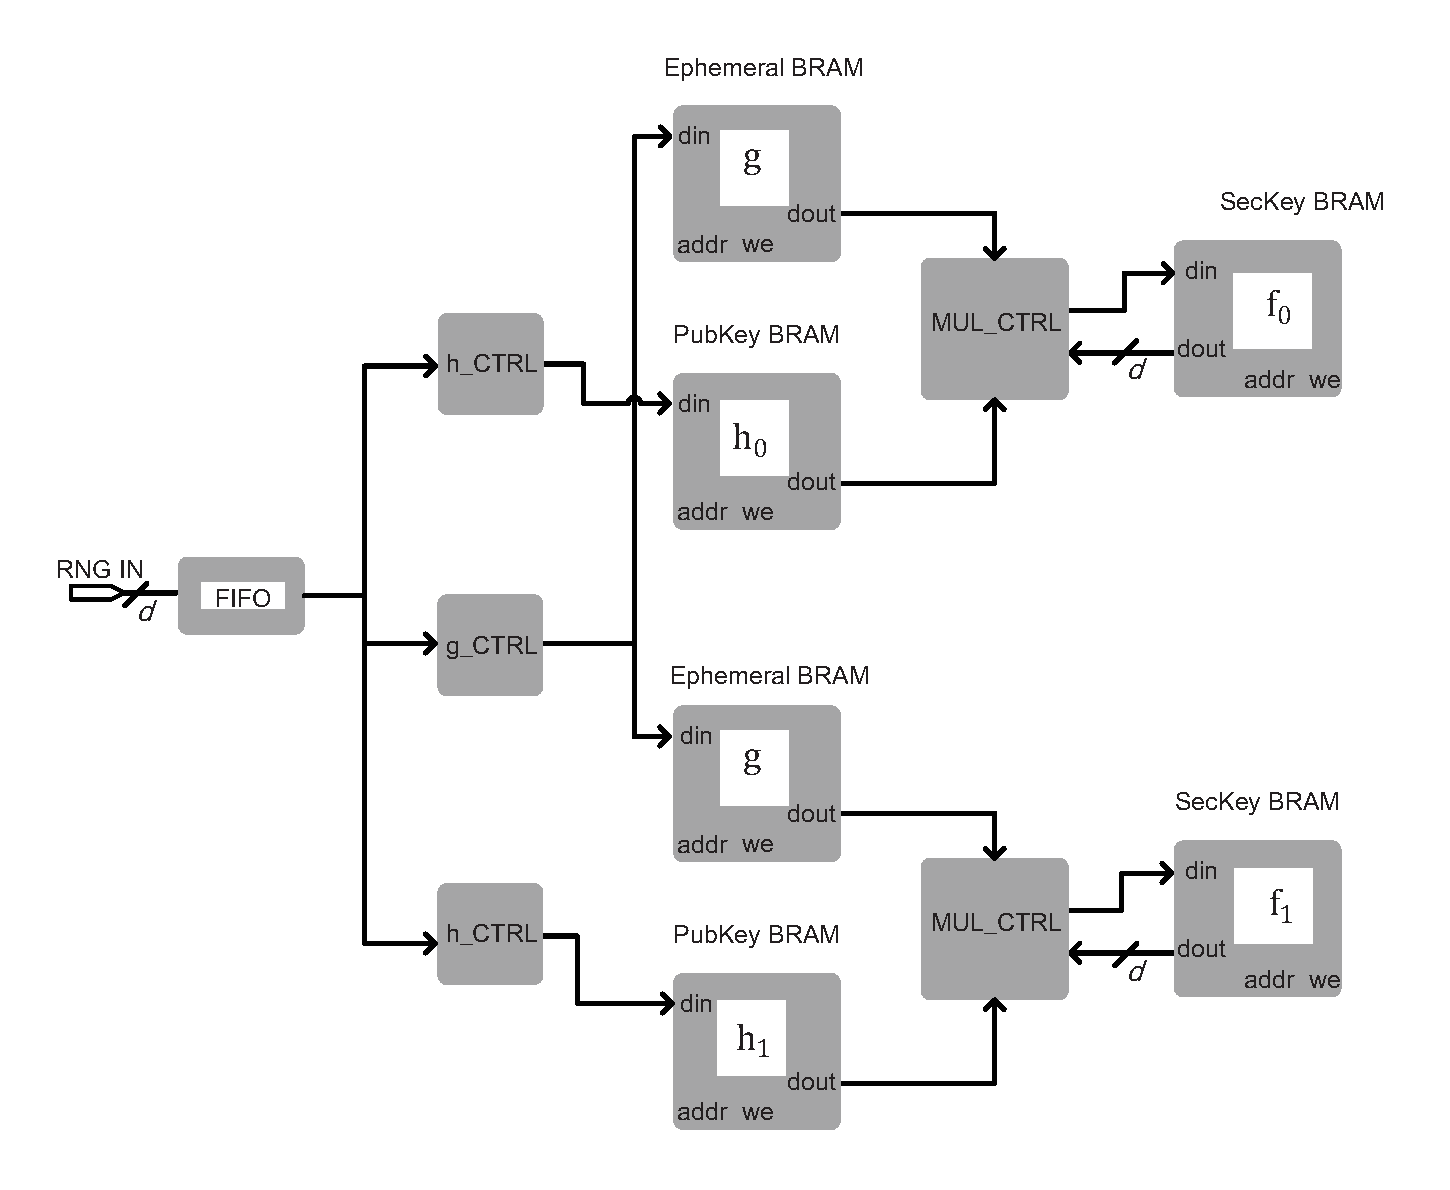
\includegraphics[width=\textwidth]{./fig/BIKE-1.eps}
\caption{BIKE-1}
\label{fig:bike1}
\end{subfigure}
\hspace{1em}
\begin{subfigure}[t]{0.47\textwidth}\centering
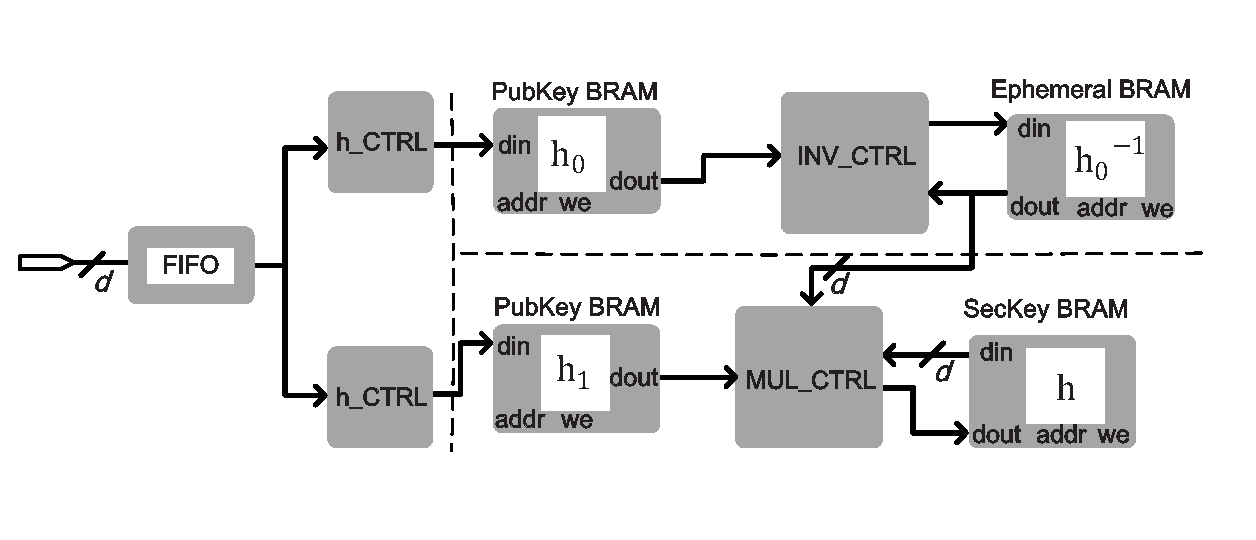
\includegraphics[width=\textwidth]{./fig/BIKE-2.eps}
\caption{BIKE-2 }
\label{fig:bike2}
\end{subfigure}
\begin{subfigure}[t]{0.47\textwidth}\centering
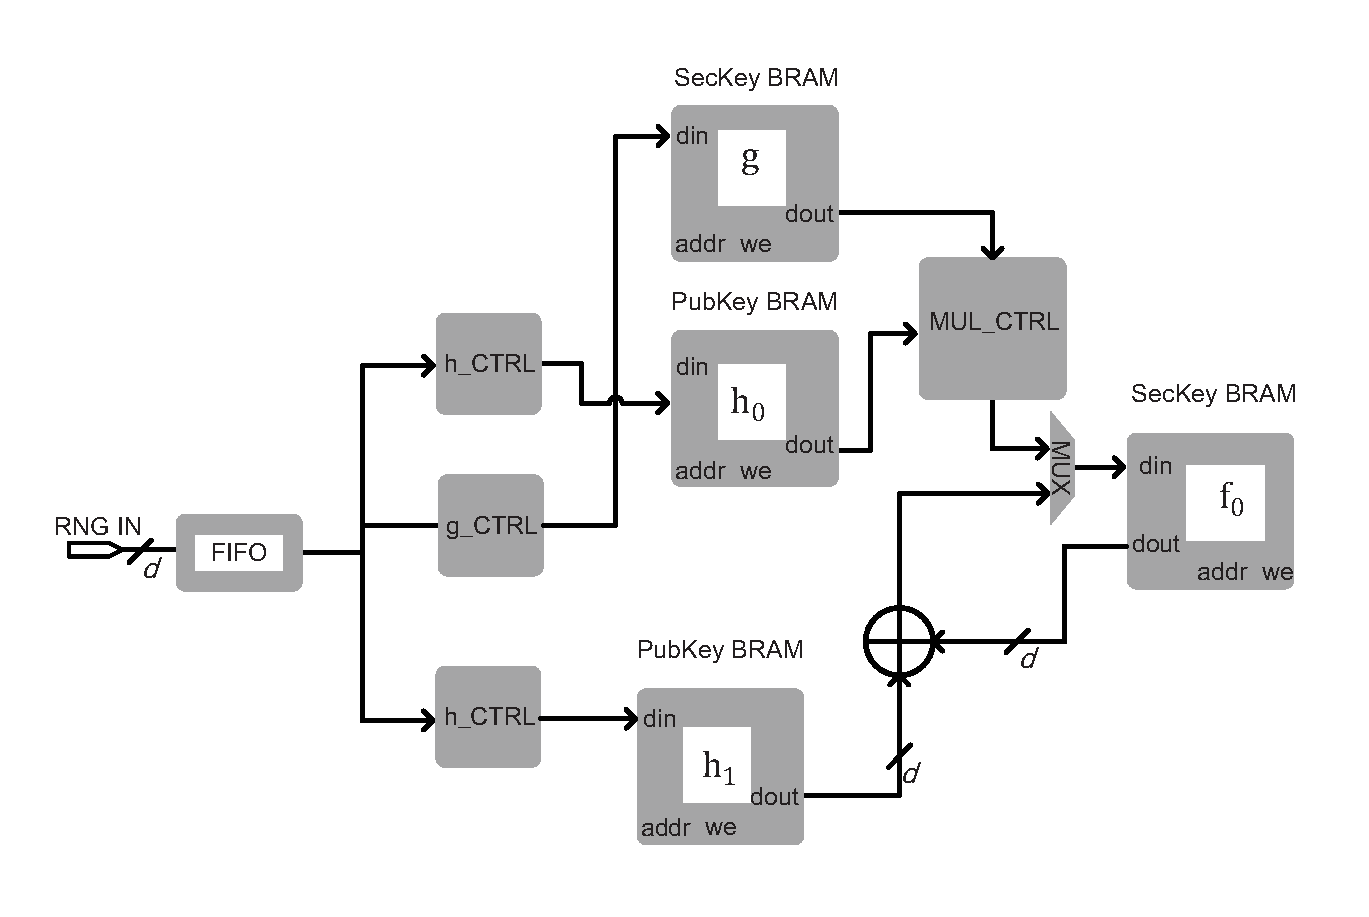
\includegraphics[width=\textwidth]{./fig/BIKE-3.eps}
\caption{BIKE-3 }
\label{fig:bike3}
\end{subfigure}
\caption{Overview of the proposed BIKE architectures}
\end{figure*}

Our key generator performs the computations in BIKE-1/2/3 as shown in Algorithm~\ref{alg:bike1_keygen}, Algorithm~\ref{alg:bike2_keygen}, and Algorithm~\ref{alg:bike3_keygen}. The top-level architectures are depicted in Figure~\ref{fig:bike1}, \ref{fig:bike2}, \ref{fig:bike3}
respectively.
BIKE-1 and BIKE-3 share similar architectures
where the sparse polynomial multiplication module
(SMUL\_CTRL in Section~\ref{sub::sparse}) is the core building block.
The difference within the two architectures is that
BIKE-1 requires two SMUL\_CTRL modules
whereas BIKE-3 requires only one SMUL\_CTRL module and one additional
addition unit.
In our design, the two sparse polynomial multiplications
in BIKE-1 are performed in parallel to improve the
timing efficiency.
Therefore, the total cycle count of BIKE-1
is close to that of BIKE-3.
Among BIKE-1/2/3, the architecture of BIKE-3 is
the most compact while the critical path is the shortest,
this is mainly due to the simplicity of the architecture
since only one SMUL\_CTRL is instantiated in BIKE-3.
The modules h\_ctrl and g\_ctrl in BIKE-3 represents the
control logic for
generating the sparse polynomials $h_0,h_1$ and
the dense polynomial $g$, as discussed in Section~\ref{sub::polygen}.

The key generator architecture for BIKE-2
is significantly more expensive compared to
BIKE-1 and BIKE-3.
This is mainly due to the requirement of a
polynomial inversion step in the key generation process,
therefore a INV\_CTRL as described in Section~\ref{sub::inversion} is needed.
% INV\_CTRL consists of the arithmetic core for continuous square and generic multiplication as illustrated in Section 2.3 and 2.4.
After the inversion operation, the inversed polynomial of
$h_0$ is obtained, which is represented as $h_0^{-1}$.
Then, the sparse polynomial multiplication begins
by triggering the SMUL\_CTRL module with polynomials
$h_0^{-1}$ and $h_1$ as inputs.
After the SMUL\_CTRL module finishes,
the result is sent out as the output,
which is the secret key $h=h_0^{-1}h_1$.
% After inversion, the dense polynomial $h_0^{-1}$ is obtained and finally, the sparse polynomial multiplication is performed on SMUL\_CTRL to extract the secret key $h=h_0^{-1}h_1$.

Similar optimizations as proposed to schedule pipelines
as described in Section~3 are applied to the
modules within the BIKE key generator as well:
% optimization technique is applied to
g\_ctrl, h\_ctrl, SMUL\_CTRL, and INV\_CTRL.
These optimizations improves the timing efficiency for the
key generator.
% The optimized piepline schedules are depicted in Figure~\ref{fig:pipeline_squ2},
% ~\ref{fig:pipeline_mul2}, and \ref{fig:pipeline_rng3}.
% As dual-port RAM is instantiated, we are able to load two successive data from secret/public keyRAM in one clock cycle to slice registers for fast processing.



\section{Performance Evaluations}
\label{sec::evaluation}

\begin{table*}[!t]\centering
 \caption{Implementation results of BIKE on a Xilinx Virtex-7 XC7V585T FPGA and a Xilinx Spartan-7 XC7S50 FPGA after the place and route process.}
 \label{table:expresult}\centering
 \begin{minipage}{\textwidth}\centering
  \begin{tabular}{lcccccc}
   \hline
   Aspect & \multicolumn{2}{c}{BIKE-1 KeyGen} & \multicolumn{2}{c}{BIKE-2 KeyGen} & \multicolumn{2}{c}{BIKE-3 KeyGen}\\
    & Virtex-7 & Spartan-7  & Virtex-7 & Spartan-7  & Virtex-7 & Spartan-7\\
   \hline
   FFs &1055   &993  &2159 &2098 &955 &911\\
   LUTs & 1970  &1897  &4445 &3872&1482&1402  \\
   Slices& 612 &544  &1483 &1272&472&423  \\
   BRAM & 7  &7  &10 & 10& 4&4\\
   \hline
   Frequency &  350 MHz  & 160 MHz &320 MHz & 150 MHz  & 360 MHz & 200 MHz\\
   Time/Op &  0.273 $ms$ &  0.597 $ms$ & 6.719 $ms$& 14.334 $ms$ &0.273 $ms$  & 0.492 $ms$\\
   \hline
   Compute $h_0$ & \multicolumn{2}{c}{$1279$ cycles} & \multicolumn{2}{c}{$1279$ cycles}  & \multicolumn{2}{c}{$1062$ cycles}\\
   Compute $h_1$& \multicolumn{2}{c}{$1279$ cycles} & \multicolumn{2}{c}{$1279$ cycles} & \multicolumn{2}{c}{$1062$ cycles}\\
   Compute $g$ & \multicolumn{2}{c}{$2068$ cycles} & \multicolumn{2}{c}{---} & \multicolumn{2}{c}{$2250$ cycles}\\
   Compute ${h_0}^{-1}$ & \multicolumn{2}{c}{---} & \multicolumn{2}{c}{$2,056,683$ cycles} &\multicolumn{2}{c}{---}\\
   Compute $f_0$ & \multicolumn{2}{c}{$90,880$ cycles} & \multicolumn{2}{c}{---} &\multicolumn{2}{c}{$94,135$ cycles}\\
   Compute $f_1$ & \multicolumn{2}{c}{$90,880$ cycles}  & \multicolumn{2}{c}{---} &\multicolumn{2}{c}{---}\\
   Compute $h$  &  \multicolumn{2}{c}{---}          & \multicolumn{2}{c}{$90,880$ cycles} & \multicolumn{2}{c}{---}\\
   \hline
   Overall & \multicolumn{2}{c}{$95,506$ cycles} & \multicolumn{2}{c}{$2,150,121$ cycles} & \multicolumn{2}{c}{$98,509$ cycles}\\
   \hline
  \end{tabular}
  \end{minipage}
\vspace{-4mm}
\end{table*}
%
In this section, we present the hardware implementation results of the
key generator of BIKE on FPGAs.
All the results are obtained post place-and-route for a
Xilinx high-end FPGA device --- Virtex XC7V585T
and a low-end FPGA device --- Spartan XC7S50 FPGA
using the Xilinx Vivado v2018.1 synthesis tool.
% which demonstrate the time and the area efficiency of our design on both platforms.
To the best of our knowledge, this work is the first
that reports the performance results of the BIKE key generator
on FPGA platforms.

As shown in Table~\ref{table:expresult},
for our BIKE-1 key generator,
when the design is synthesized on the Virtex-7 device,
the synthesis tool reports a maximum frequency of 350~MHz.
Our simulation result shows that it takes $95,506$ cycles
to generate one key pair for BIKE-1.
Therefore, to generate a complete key pair for BIKE-1,
only 0.273 $ms$ are needed.
When synthesized for a lower-end Spartan-7 device,
our design is reported to be able to run at 160~MHz
which leads to a key pair generation time of 0.597~$ms$.
The area consumption of the key generator
for BIKE-1 is very low: Only 612 slices and 544 slices
are needed on Virtex-7 and Spartan-7 respectively.
% as our proposed architecture uses the proposed optimized sparse polynomial multiplication, and executes all operations in word level (here in this concrete experiment, 64-bits of data are operated per time), which costs limited hardware resources.
Compared to BIKE-1, the key generator for BIKE-3
is more compact since only one sparse polynomial
multiplication module is needed instead of two.
However, BIKE-3 takes slightly more cycles
compared to BIKE-1 to generate a key pair
due to the additional polynomial addition operation
needed for computing the secret key $f_0$
in BIKE-3.
In terms of run time,
the performance of the BIKE-3 key generator
is slightly better than BIKE-1:
The key pair generation take $0.273$ $ms$ and $0.492$ $ms$
respectively on Virtex-7 and Spartan-7 FPGAs.
% The slice overheads are also lower as BIKE-3 carries one copy of the core unit, sparse polynomial multiplication whereas BIKE-1 has two of them. The cycle count is slightly worse than that of BIKE-1 as BIKE-3 requires an extra polynomial addition to compute the secret key $f_0$.

For the BIKE-2 key generator, the synthesis tool reports
frequencies as 320 MHz and 150 MHz on the Virtex-7 and Spartan-7 devices respectively.
A full key generation in BIKE-2 takes $2,150,121$ cycles
which leads to run time of $6.719$ ms and $14.334$ ms respectively
on Virtex-7 and Spartan-7 devices.
As we can see from Table~\ref{table:expresult},
BIKE-2 is around two orders of magnitude slower compared to BIKE-1 and BIKE-3.
This performance gap between BIKE-2 and BIKE-1/3 is mainly
due to the requirement of an expensive polynomial inversion operation in BIKE-2
while in BIKE-1/3 it is not needed.
% Nevertheless, by using the proposed generic multiplication algorithm and continuous square algorithm, the BIKE-2 timing is significantly improved and preserves the constant-time execution.
Due to the existance of the polynomial inversion module,
the area utilization of BIKE-2 key generator is more than $2\times$
bigger compared to BIKE-1/3 as well.
% The slice usage is also conservative, increasing by 2-3 times compared with BIKE-1 and BIKE-2.
Moreover, the memory overhead in BIKE-2 key generator
is also larger than that of BIKE-1/3 since
the polynomial inversion module
requests to save a few ephemeral variables.

\section{Related Work}
In the following, we compare our work with previous designs.
% \paragraph{Hardware Architectures for Goppa Code-based Cryptosystems.}
Hardware architectures for the classical McEliece/Niederreiter
schemes based on binary Goppa
codes have been extensively studied in the last decade
~\cite{eisenbarth2009microeliece,shoufan2010novel,ghosh2012speed,heyse2012towards,wang2017fpga,wang2018fpga}.
In 2018, Wang, Niederhagen and Szefer presented
the fastest-to-date FPGA-based design for the
Goppa code-based Niederreiter cryptosystem~\cite{wang2018fpga}
which includes all the operations, i.e.,
key generation~\cite{wang2017fpga}, encryption and decryption.
As we can see from Table~\ref{table:compare}, with the same security level,
cryptosystems based on binary Goppa codes
require much more time, slices and memory to generate
a key pair.
Such memory overhead is inevitable in Goppa code
cryptosystems due to its large public key size
which does not exisit in cryptosystems based on
quasi-cyclic codes.
 % as Goppa code cannot benefit from quasi-cyclic construction to compress the key size.
Therefore, compared to binary Goppa code-based key generatos,
our design based on QC MDPC codes is a much more lightweight
design which is also much more efficient and has a
much smaller memory overhead.

% Their design generates a key pair in $3.98 ms$ for 256-bit security on an Ultrascale+ FPGA.

% First, we compare our work with a hardware design from [17], which
% presents the previously fastest decryption module for a McEliece cryptosystem. Therefore the comparison of our work with design [17] focuses on the
% decryption part. We synthesized our decryption module with the parameters
% they used, which correspond to a 128-bit classical security level, for a Virtex-6
% XC6VLX240T FPGA.
% In 2009, the first FPGA-based implementation of the McEliece cryptosystem was proposed based on
% a Spartan-3 FPGA.
% The encryption and decryption operations are finished in 1.07 ms and 2.88 ms,
% using security parameters achieving an equivalence of 80-bit classical security~\cite{eisenbarth2009microeliece}.
% The authors of~\cite{shoufan2010novel} presented an improved design for the McEliece cryptosystem
% with a similar level of security.
% The design in~\cite{shoufan2010novel} is based on a more powerful Virtex-5 FPGA,
% and is capable to encrypt and decrypt in 0.5 ms and 1.3 ms respectively.
% Another work~\cite{ghosh2012speed} based on the
% hardware/software co-design of the McEliece cryptosystem
% is based on a Spartan-3 FPGA and decrypts a ciphertext in 1 ms at
% 92 MHz with
% 80-bit security.
% Later, Heyse and G\"uneysu~\cite{heyse2012towards} in 2012 report
% that the decryption operation of the Niederreiter cryptosystem
% takes 58.78 $\mu$s on a Virtex-6 FPGA
% with 80-bit security.

A few hardware designs have been proposed on MDPC code-based
cryptosystems~\cite{heyse2013smaller,von2014lightweight,hu2017area}.
However, all of these designs only focus on the encryption/decryption
operations in the cryptosystem.
Therefore, a direct comparison of our work
with other key generator architectures of MDPC code-based
cryptosystems are not feasible.
% The first implementation of MDPC code-based McEliece cryptosystem on FPGAs
% was presented in~\cite{heyse2013smaller} in 2013.
% For 80-bit security, it is reported to run decryption in 125 $\mu$s
% with over 10,000 slices on a Virtex-6 FPGA.
% A more lightweight version of the same cryptosystem has been implemented
% on FPGAs by sequentially manipulating cyclic rotations of the private key in block RAMs~\cite{von2014lightweight}.
% This lightweight design is very compact and costs only 64 slices for encryption and
% 148 slices for decryption on a low-end Spartan-6 device.
% An area-time efficient MDPC code-based Niederreiter cryptosystem has been proposed~\cite{hu2017area}
% by exploiting an efficient MDPC decoding unit.
% Their experimental results show that their hardware architecture is able to decrypt a
% ciphertext in 65 $\mu$s by using about 8,000 slices on a Virtex-6 FPGA.

To get a better comparison with other work on MDPC code-based cryptosystems,
we also compared our work with the state-of-the-art software implementations of BIKE.
% on either CPUs or micro-controllers.
Note that a fair comparison between our hardware design and other software implementations
of BIKE is not feasible since the platforms are fully different.
% We attempt to compare the performance in the metric of cycle count which is a platform independent indicator, given in Table \ref{table:compare}.
Comparison results are provided in Table~\ref{table:compare}.
We first compare our design with the implementation
which is included in the BIKE specification
submitted to the NIST 2nd round PQC standardization process~\cite{aragon2017bike}.
% standard BIKE specification implementation \cite{aragon2017bike} which is also submitted for NIST PQC standardization.
% The experiments from \cite{von2014lightweight} is equipped with an Intel i5 CPU running at 1.8 GHz and 32 GB RAM, 32K L1d and L1i cache, 256K L2 cache, and 4096K L3 cache.
As we can see from Table~\ref{table:compare}, with the same security levels,
for BIKE-1, our design is around $7.7\times$ faster than their implementation
in terms of cycle count.
Moreover, the software implementation provided in~\cite{aragon2017bike} is not constant-time and
therefore is vulerable to timing side-channel attacks.
% is much slower than ours.
% The micro-controller implementation from \cite{maurich2015implementing} is performed on ARM Cortex-M4 and uses obsolete BIKE-2 system parameters with 80-bit security level which is not recommended in the NIST PQC standardization. Despite the insufficiently 80-bit SL parameters used in \cite{maurich2015implementing}, their implementation is non-constant time and costs huge cycle count (148.5 million).
An optimized software implementation for BIKE is reported in~\cite{drucker2017toolbox}.
% This additional implementation is equipped with an Intel i5 CPU running at 3.0 GHz and 70 GB RAM, 32K L1d and L1i cache, 1024K L2 cache, and 25,344K L3 cache.
In this implementation,
the core functionality in BIKE is written in assembly language,
moreover, the PCLMULQDQ instruction extension is exploited
to enable carry-less multiplication to speed up
the computations in BIKE.
The performance results of~\cite{drucker2017toolbox}
is provided in Table~\ref{table:compare}.
In terms of cycle count, for BIKE-1, the performance of our hardware design is
comparable to~\cite{drucker2017toolbox} while an over $2\times$
speedup is achieved in BIKE-2.
% results are comparable and even better than \cite{drucker2017toolbox}.
% The implementation uses the PCLMULQDQ architecture extension to enable carry-less multiplication for performance gain. Despite these dedicate and platform-dependent optimizations, our results are comparable and even better than \cite{drucker2017toolbox}. The performance gain of our design comes from two aspects: first, the pipelining parallelization is proposed for core functions including squaring, multiplication. second, the proposed continuous squaring, generic multiplication, and sparse polynomial multiplication has lower communication overheads to external memory which facilitate computational accelerations on FPGA.



\begin{table*}[!t]\centering
\caption{Performance comparison of our FPGA implementation with dedicate software implementations.}
\label{table:compare}
\begin{minipage}{\textwidth}\centering
\scalebox{1.0}{\begin{tabular}{lcccc}
\hline
Scheme &{SL [bit]}&  Implementation & Platform & \tabincell{c}{Performance\\{} [in millions of cycles]}\\
\hline
\multirow{3}{*}{\textbf{BIKE-1}} & 128 & Ours, constant-time & FPGA & 0.095\\
                                & 128 & \cite{aragon2017bike}, non-constant-time & {Intel Core-i5} & $\approx 0.73$\\
                                & 128 & \cite{drucker2017toolbox}, non-constant-time & {Intel Xeon-8124M} & 0.09\\
\hline
\multirow{3}{*}{\textbf{BIKE-2}} & 128 & Ours, constant-time & FPGA & 2.15\\
                                & 128 & \cite{aragon2017bike}, non-constant-time & {Intel Core-i5} &$\approx 6.3$\\
                                & 128 & \cite{drucker2017toolbox}, non-constant-time & {Intel Xeon-8124M} & 4.38\\
                                 % & 80 & \cite{maurich2015implementing} & Micro-controller &$\approx 148.5$\\
\hline
\multirow{2}{*}{\textbf{BIKE-3}} & 128 & Ours, constant-time & FPGA & 0.098\\
                                 & 128 & \cite{aragon2017bike}, non-constant-time & {Intel Core-i5} &$\approx 0.43$ \\
\hline
\end{tabular}}
\end{minipage}
\vspace{-4mm}
\end{table*}


\begin{table*}[!t]\centering
\caption{Performance comparison of our FPGA implementation with other code-based key generators.}
\label{table:compare}
\begin{minipage}{\textwidth}\centering
\scalebox{0.9}{\begin{tabular}{lcccccccc}
\hline
Scheme &\tabincell{c}{SL\\{} [bit]}&Platform &$f$[MHz] & Time/Op & Cycles  & Slices & BRAM\\
\hline
MDPC code:\\
\textbf{Ours (BIKE-1)} & \multirow{3}{*}{\textbf{128}} & \multirow{3}{*}{Virtex-7} & {\textbf{350}}  & $\mathbf{0.273 ms}$& $9.55\times 10^4$  & \textbf{612} & \textbf{7}\\
\textbf{Ours (BIKE-2)} &  &  & {\textbf{320}}  & $\mathbf{6.719 ms}$& $2.15\times 10^6$  & \textbf{1483} & \textbf{10}\\
\textbf{Ours (BIKE-3)} &  &  & {\textbf{360}}  & $\mathbf{0.273 ms}$& $9.85\times 10^4$  & \textbf{472} & \textbf{4}\\
\hline
Goppa code:\\
\cite{wang2018fpga} &{256} &{Virtex Ultrascale+} & {225}   & $3.98ms$    & $\approx 1.01\times 10^{11}$  & {112,845}& {375}\\
\cite{wang2018fpga} &{103} &{Virtex 5} & {168}   & $16 ms$    & $\approx 2.72\times 10^6$  & {8171}& {89}\\
% \cite{shoufan2010novel} &{103} &{Virtex 5} & {163}   & $90 ms$    & $\approx 1.47\times 10^7$  & {17,280}& {148}\\
\hline
\end{tabular}}
\end{minipage}
\vspace{-4mm}
\end{table*}

% Second, we compare our work with other existing hardware solutions based on Goppa codes \cite{wang2018fpga,shoufan2010novel}. As the state-of-art reference, we consider the implementation reported in \cite{wang2018fpga}, where scalability is tested with different system parameters and FPGA platforms. We extract from \cite{wang2018fpga} the experimental results at 256-bit SL and 103-bit SL on Xilinx FPGAs to provide a direct and fair comparison.
% It is seen that for almost the same security level, Goppa codes require much more memory and computation time to generate the public/secret key. Such memory overhead is inevitable in Goppa code schemes as Goppa code cannot benefit from quasi-cyclic construction to compress the key size.
% Conversely, our work based on quasi-cyclic codes is identified as a scalable lightweight design which shares high-speed and low-storage characteristics.

 \section{Conclusions}
 \label{sec::conclusion}
 This paper presented a constant-time hardware-based key generator for BIKE which is among the
 2nd round candidate in the NIST PQC standardization process.
 Novel multiplication and squaring algorithms were proposed to accelerate the key generation with low logic overhead. Experimental results show that after a dedicate optimized pipeline scheduling for the proposed algorithms, our work outperforms other code-based hardware key generators in terms of timing performance, logic utilization and memory consumption. This work even beats software implementations with powerful CPUs in terms of cycle count. The methods proposed in this paper are generic and applicable to other code-based schemes if the underlying code is quasi-cyclic.

%
% ---- Bibliography ----
%
% BibTeX users should specify bibliography style 'splncs04'.
% References will then be sorted and formatted in the correct style.
%
% \bibliographystyle{splncs04}
% \bibliography{mybibliography}
%
\bibliographystyle{abbrv}
\bibliography{./reference}

\newpage

\section*{Appendix}
%

\subsection{Illustrative example for constant-time ITA used in BIKE}
We illustrate a concrete instance for computing the polynomial inversion used in BIKE-2 as shown in Table~\ref{table:ita_example}. 

\begin{table}[!tb]\centering
\caption{An illustrative example for computing polynomial inverse $a^{-1}$ in $\mathbb{F}_2[x]/(x^r+1)$ with $r=10163$ used in BIKE-2. This table explicitly demonstrates step by step a constat-time execution for inverse.}
\label{table:ita_example}
\begin{tabular}{ccccc}
  \hline
  % after \\: \hline or \cline{col1-col2} \cline{col3-col4} ...
  $i$ & $u_i$ & rule & $[\beta_{u_{i_1}}(a)]^{2^{u_{i_2}}}\cdot \beta_{u_{i_2}}(a)$ & $\beta_{u_{i_i}}(a)=a^{2^{u_i}-1}$\\
  \hline
  0   & 1       & --- & ---                                                         & $\beta_{u_{i_0}}(a)=a^{2^{1}-1}$\\
  1   & 2       & $2u_{i-1}$ &$[\beta_{u_{i_0}}(a)]^{2^{u_{i_0}}}\cdot \beta_{u_{i_0}}(a)$ & $\beta_{u_{i_1}}(a)=a^{2^{2}-1}$\\
  2   & 4       & $2u_{i-1}$ &$[\beta_{u_{i_1}}(a)]^{2^{u_{i_1}}}\cdot \beta_{u_{i_1}}(a)$ & $\beta_{u_{i_2}}(a)=a^{2^{4}-1}$\\
  3   & 8       & $2u_{i-1}$ &$[\beta_{u_{i_2}}(a)]^{2^{u_{i_2}}}\cdot \beta_{u_{i_2}}(a)$ & $\beta_{u_{i_3}}(a)=a^{2^{8}-1}$\\
  4   & 9  & $u_{i-1}+u_0$   &$[\beta_{u_{i_3}}(a)]^{2^{u_{i_0}}}\cdot \beta_{u_{i_0}}(a)$ & $\beta_{u_{i_4}}(a)=a^{2^{9}-1}$\\
  5   & 18       & $2u_{i-1}$ &$[\beta_{u_{i_4}}(a)]^{2^{u_{i_4}}}\cdot \beta_{u_{i_4}}(a)$ & $\beta_{u_{i_5}}(a)=a^{2^{18}-1}$\\
  6   & 19  & $u_{i-1}+u_0$   &$[\beta_{u_{i_5}}(a)]^{2^{u_{i_0}}}\cdot \beta_{u_{i_0}}(a)$ & $\beta_{u_{i_4}}(a)=a^{2^{19}-1}$\\
  7   & 38  & $2u_{i-1}$ &$[\beta_{u_{i_6}}(a)]^{2^{u_{i_6}}}\cdot \beta_{u_{i_6}}(a)$ & $\beta_{u_{i_7}}(a)=a^{2^{38}-1}$\\
  8   & 39  & $u_{i-1}+u_0$   &$[\beta_{u_{i_7}}(a)]^{2^{u_{i_0}}}\cdot \beta_{u_{i_0}}(a)$ & $\beta_{u_{i_8}}(a)=a^{2^{39}-1}$\\
  9   & 78  & $2u_{i-1}$ &$[\beta_{u_{i_8}}(a)]^{2^{u_{i_8}}}\cdot \beta_{u_{i_8}}(a)$ & $\beta_{u_{i_9}}(a)=a^{2^{78}-1}$\\
  10  & 79  & $u_{i-1}+u_0$   &$[\beta_{u_{i_9}}(a)]^{2^{u_{i_0}}}\cdot \beta_{u_{i_0}}(a)$ & $\beta_{u_{i_{10}}}(a)=a^{2^{79}-1}$\\
  11  & 158  & $2u_{i-1}$ &$[\beta_{u_{i_{10}}}(a)]^{2^{u_{i_{10}}}}\cdot \beta_{u_{i_{10}}}(a)$ & $\beta_{u_{i_{11}}}(a)=a^{2^{158}-1}$\\
  12  & 316  & $2u_{i-1}$ &$[\beta_{u_{i_{11}}}(a)]^{2^{u_{i_{11}}}}\cdot \beta_{u_{i_{11}}}(a)$ & $\beta_{u_{i_{12}}}(a)=a^{2^{316}-1}$\\
  13  & 317  & $u_{i-1}+u_0$   &$[\beta_{u_{i_{12}}}(a)]^{2^{u_{i_0}}}\cdot \beta_{u_{i_0}}(a)$ & $\beta_{u_{i_{13}}}(a)=a^{2^{317}-1}$\\
  14  & 634  & $2u_{i-1}$ &$[\beta_{u_{i_{13}}}(a)]^{2^{u_{i_{13}}}}\cdot \beta_{u_{i_{13}}}(a)$ & $\beta_{u_{i_{14}}}(a)=a^{2^{634}-1}$\\
  15  & 635  & $u_{i-1}+u_0$   &$[\beta_{u_{i_{14}}}(a)]^{2^{u_{i_0}}}\cdot \beta_{u_{i_0}}(a)$ & $\beta_{u_{i_{15}}}(a)=a^{2^{635}-1}$\\
  16  & 1270  & $2u_{i-1}$ &$[\beta_{u_{i_{15}}}(a)]^{2^{u_{i_{15}}}}\cdot \beta_{u_{i_{15}}}(a)$ & $\beta_{u_{i_{16}}}(a)=a^{2^{1270}-1}$\\
  17  & 2540  & $2u_{i-1}$ &$[\beta_{u_{i_{16}}}(a)]^{2^{u_{i_{16}}}}\cdot \beta_{u_{i_{16}}}(a)$ & $\beta_{u_{i_{17}}}(a)=a^{2^{2540}-1}$\\
  18  & 5080  & $2u_{i-1}$ &$[\beta_{u_{i_{17}}}(a)]^{2^{u_{i_{17}}}}\cdot \beta_{u_{i_{17}}}(a)$ & $\beta_{u_{i_{18}}}(a)=a^{2^{5080}-1}$\\
  19  & 10160 & $2u_{i-1}$ &$[\beta_{u_{i_{18}}}(a)]^{2^{u_{i_{18}}}}\cdot \beta_{u_{i_{18}}}(a)$ & $\beta_{u_{i_{19}}}(a)=a^{2^{10160}-1}$\\
  20  & 10161 & $u_{i-1}+u_0$ &$[\beta_{u_{i_{19}}}(a)]^{2^{u_{i_{0}}}}\cdot \beta_{u_{i_{0}}}(a)$ & $\beta_{u_{i_{20}}}(a)=a^{2^{10161}-1}$\\
  \hline
\end{tabular}
\end{table}

\subsection{Proof of Theorem~1}
We briefly proof Theorem~1 as follows:
Consider the straighforward squaring operation for a random polynomial $a(x)\in \mathcal{R}$:
\begin{align}
    a^2(x) &= (a_{r-1}x^{r-1}+a_{r-2}x^{r-2}+\cdots + a_{1}x + a_0)^2\\
    &= a_{r-1}x^{2(r-1)}+a_{r-2}x^{2(r-2)}+\cdots + a_1x^2 + a_0\\
    &= \widetilde{a_{r-1}}x^{r-1}+\widetilde{a_{r-2}}x^{r-2}+\cdots + \widetilde{a_{1}}x +\widetilde{a_0}
\end{align}
%
The computation of the coefficients $\widetilde{a_{i}}$ can
be realized by a matrix multiplication operation,
which relies on the base transformation matrix BT, as shown follows:
\[
a^2(x)= [{a_{0}},{a_{1}},\cdots,{a_{r-1}}]\left[ \begin{array}{c}
x^{0} \\
x^{2} \\
\vdots\\
x^{2(r-2)}\\
x^{2(r-1)}
\end{array}
\right ]
=
[{a_0},{a_1},\cdots,{a_{r-1}}]
\cdot \text{BT}_{r\times r} \cdot
\left[ \begin{array}{c}
x^{0} \\
x^{1} \\
\vdots\\
x^{r-2}\\
x^{r-1}
\end{array}
\right ]
\]
where $[\widetilde{a_{0}},\widetilde{a_{1}},\cdots,\widetilde{a_{r-1}}]=[{a_{0}},{a_{1}},\cdots,{a_{r-1}}]
\cdot \text{BT}$ and BT is a $r\times r$ permutation matrix defined as:
\[
\text{BT} =
\left[ \begin{array}{ccccc}
\mathbf{1}_{0}&0&\cdots&\cdots&\cdots  \\
\cdots&\mathbf{1}_{2}&0 &\cdots&\cdots \\
\vdots&\vdots&\vdots&\vdots&\vdots\\
\vdots&\vdots&\mathbf{1}_{2r-4}&0&\vdots\\
\vdots&\vdots&\vdots&\mathbf{1}_{2r-2}&0\\
\end{array}
\right ]
\]
$\mathbf{1}_{i}$ represents the ($i\bmod r$)-th (counting from zero) non-zero entry in the corresponding row of the matrix BT.
%
More generally, we derive the base transformation matrix $\text{BT}_n=\text{BT}^n$ for
computing polynomial squaring continuously:
$a(x)^{2^n}=\widetilde{a_{r-1}}x^{r-1}+\widetilde{a_{r-2}}x^{r-2}+\cdots + \widetilde{a_{1}}x +\widetilde{a_0}$.
As we will see in Section~\ref{sub::inversion},
this is particularly useful in computing the
inverse of a polynomial.
\[
\text{BT}^n =
\left[ \begin{array}{ccccc}
\mathbf{1}_{0}&0&\cdots&\cdots&\cdots  \\
\cdots&\mathbf{1}_{2^n}&0 &\cdots&\cdots \\
\vdots&\vdots&\vdots&\vdots&\vdots\\
\vdots&\vdots&\mathbf{1}_{(r-2)2^n}&0&\vdots\\
\vdots&\vdots&\vdots&\mathbf{1}_{(r-1)2^n}&0\\
\end{array}
\right ]
\]
%
In order to compute the coefficient vector $[\widetilde{a_{0}},\widetilde{a_{1}},\cdots,\widetilde{a_{r-1}}]=[{a_{0}},{a_{1}},\cdots,{a_{r-1}}]
\cdot \text{BT}^n$, $\text{BT}^n$ must be represented in column view format, \textit{i.e.},
the row number of the non-zero entry for every column of $\text{BT}^n$. In this form, the squaring of $a(x)$ is essentially the substitutions of the coefficients of $a(x)$:
\[
\text{BT}^n =
\left[ \begin{array}{ccccc}
\mathbf{1}_{0}&\vdots& \vdots&\vdots&\vdots \\
\vdots&\mathbf{1}_{2^{-n}}&\vdots&\vdots&\vdots\\
\vdots&\vdots&\vdots&\mathbf{1}_{(r-2)2^{-n}}&\vdots\\
\vdots&\vdots&\vdots&\vdots&\mathbf{1}_{(r-1)2^{-n}}\\
\end{array}
\right ]
\]


\subsection{Remarks on generic multiplication}
We describe the proposed generic multiplication algorithm (Alg.~\ref{alg:generic_mul}) in more details here. Similar to the proposed squaring algorithm,
another base transformation matrix $\text{BT}_{mul}$ is used to compute the coefficients $\widetilde{c_{i}}$, shown as follows:
\[
a(x)b(x)= [\widetilde{c_{0}},\widetilde{c_{1}},\cdots,\widetilde{c_{r-1}}]\left[ \begin{array}{c}
x^{0} \\
x^{1} \\
\vdots\\
x^{r-2}\\
x^{r-1}
\end{array}
\right ]
=
[{a_{0}},{a_{1}},\cdots,{a_{r-1}}]
\cdot \text{BT}_{mul,r\times r} \cdot
\left[ \begin{array}{c}
x^{0} \\
x^{1} \\
\vdots\\
x^{r-2}\\
x^{r-1}
\end{array}
\right ]
\]
$\text{BT}_{mul}$ is a $r\times r$ matrix where each column/row is a cyclic form of the vector $[b_{r-1},b_{r-2},\ldots, b_{1},b_{0}]$:
\[
\text{BT}_{mul} =
\left[ \begin{array}{cccccc}
b_{0}&b_{1}&\cdots&b_{d-1}&\cdots &b_{r-1} \\
b_{r-1}&b_{0}&\cdots&b_{d-2}&\cdots &b_{r-2} \\
\vdots&\vdots&\vdots&\vdots&\vdots&\vdots\\
b_{2}&b_{3}&\cdots&b_{d+1}&\cdots &b_{1} \\
b_{1}&b_{2}&\cdots&b_{d}&\cdots &b_{0} \\
\end{array}
\right ]
\]

\begin{figure*}[!tb]
\centering
\begin{subfigure}[t]{0.47\textwidth}\centering
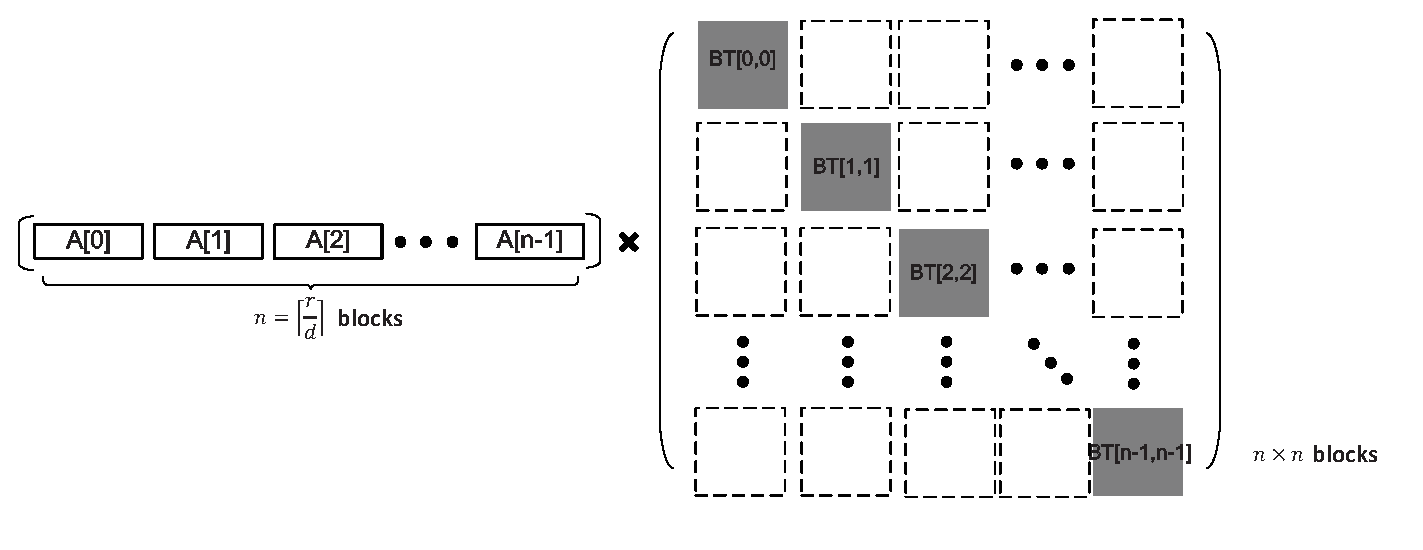
\includegraphics[width=\textwidth]{./fig/generic_mul_illustrate.eps}
\caption{Diagonal Computation}
\label{fig:gmul_ill1}
\end{subfigure}
\hspace{1em}
\begin{subfigure}[t]{0.47\textwidth}\centering
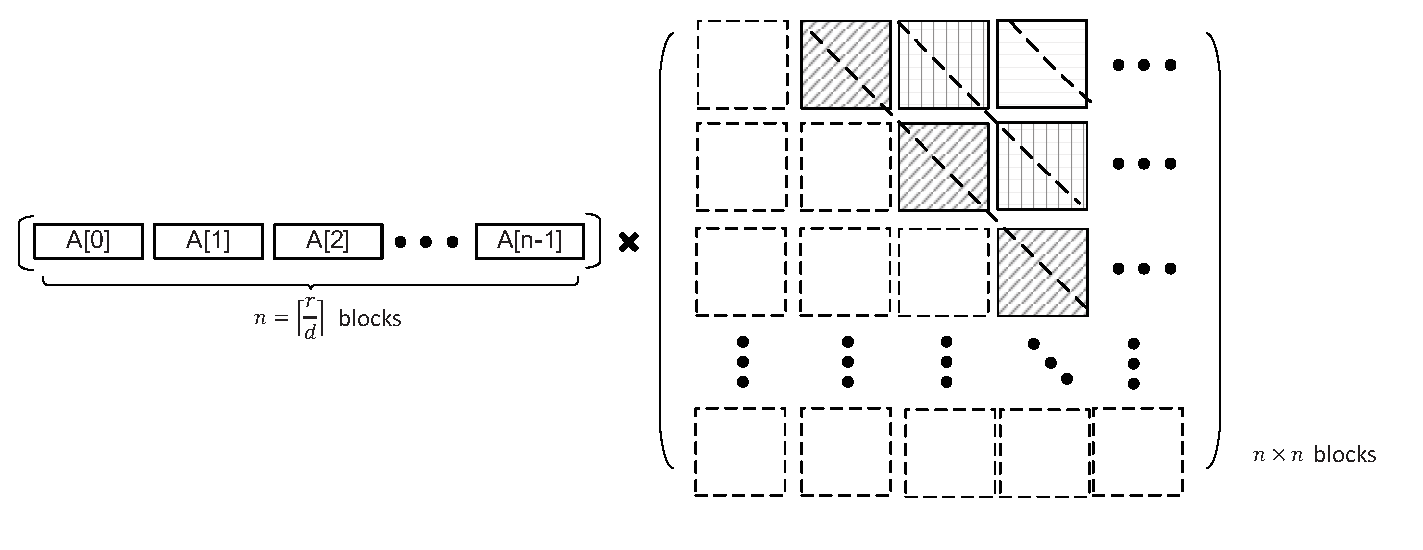
\includegraphics[width=\textwidth]{./fig/generic_mul_illustrate2.eps}
\caption{Upper Triangle Computation}
\label{fig:gmul_ill2}
\end{subfigure}
\hspace{1em}
\begin{subfigure}[t]{0.47\textwidth}\centering
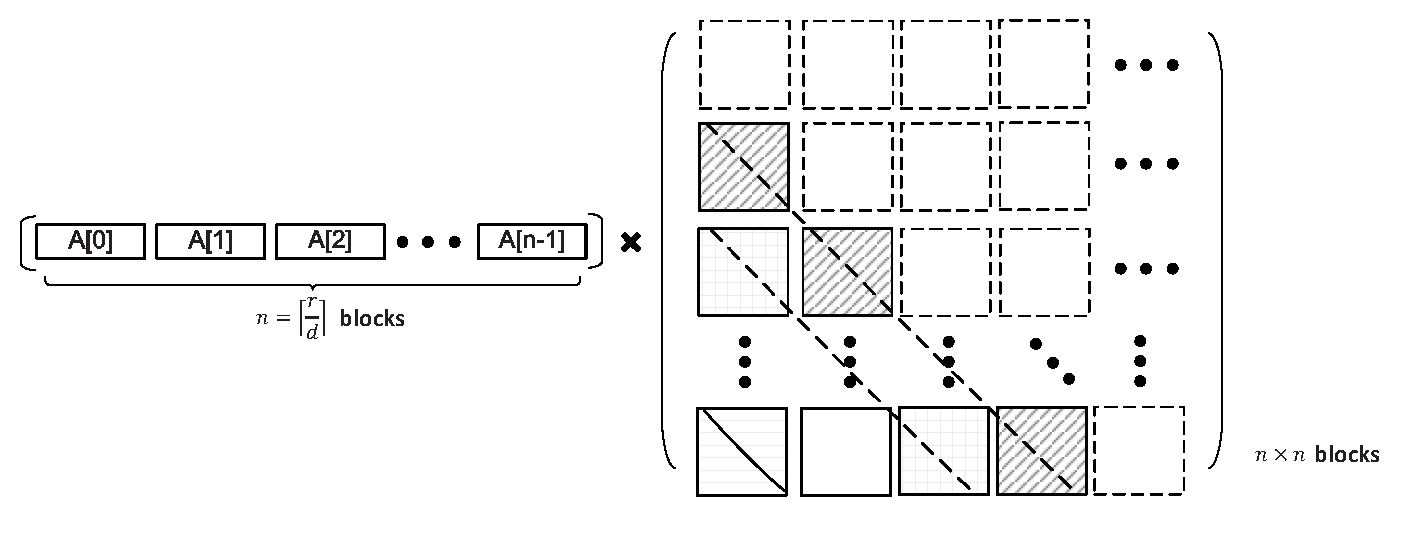
\includegraphics[width=\textwidth]{./fig/generic_mul_illustrate3.eps}
\caption{Lower Triangle Computation}
\label{fig:gmul_ill3}
\end{subfigure}
\caption{Illustration for the proposed generic multiplication algorithm}
\end{figure*}
Storing the full $\text{BT}_{mul}$ matrix is redundant
since the blocks along each diagonal are identical
(for example, $\text{BT}_{mul}[0:d-1,0:d-1] = \text{BT}_{mul}[d:2d-1,d:2d-1] = \ldots$).
This way, $\text{BT}_{mul}$ is split into three parts: the central diagonal, the upper triangle, and the lower triangle. Figure~\ref{fig:gmul_ill1}, \ref{fig:gmul_ill2}, and \ref{fig:gmul_ill3} illustrate how to compute these parts.
By eliminating such redundancy, the communication overhead for
loading $\text{BT}_{mul}$ is minimized which enables a
fast pipeline scheduling in the generic polynomial multiplication module.

\end{document}
